%%%%%%%%%%%%%%%%%%%%%%%%%%%%%%%%%%%%%%%%%%%%%%%%%%%%%%%%%%%%%
% Matt Pitkin 26/04/05                                      %
%                                                           %
% Chapter 4: What do you mean you want results ...!?        %
%%%%%%%%%%%%%%%%%%%%%%%%%%%%%%%%%%%%%%%%%%%%%%%%%%%%%%%%%%%%%
\chapquote{Facts are meaningless. You could use facts to prove anything that's even remotely
true!}{Homer Simpson - The Simpsons}
%\chapquote{Quote!}{Who by?}
%Oh, people can come up with statistics to prove anything, Kent. Forty percent of people know that.
%\chapter{Ding, ding ding goes the trolley, ring, ring, ring goes the neutron star}
\chapter{Neutron star quasi-normal mode searches}
% quick description of chapter
In this chapter we will describe the possible emission of gravitational wave ring-down signals from
neutron stars during glitches. We then describe two search techniques; one using
matched-filtering and the other using Bayesian evidence (sometimes called the marginal likelihood).
These techniques are them applied to search for a ring-down signal from the magnetar SGR\,1806-20
during a GRB on $27^{\rm th}$ December
2004.

% blah blah blah
% gravitational wave this, gravitational wave that
\section{Neutron stars as burst sources}
As well as being potential sources of continuous gravitational waves, under certain conditions
neutron stars may also provide a good source of burst-like transient events. Such bursts could come
from the birth of the neutron star in a supernova, where the violence of the event excites various
vibrational modes of the hot young proto-neutron star (PNS) \cite{AnderssonKokkotas:2005}. At
present there have been no searches to specifically target vibrational mode signals from PNSs,
although such signals could possibly come under the remit of more generic burst source searches.
Neutron stars in binary systems will emit a transient chirp signal during the final stages of the
binary inspiral as they coalesce. These are some of the most promising \gw sources as the extreme
energetics of the event can produce very large amplitude waves that can be seen over great
distances. Searches for such signals have been carried out using data from the LIGO detectors (see
Abbott {\it et al.}, 2004b \cite{Abbott2:2004}). For the current LIGO sensitivity such binary
inspiral signals (for two $1.4\,M_{\odot}$ neutron stars) will be observable out to a distance of
$\lesssim 15$\,Mpc.

There is another possible mechanism which could induce a burst of \gws from a neutron star.
Quasi-normal mode oscillations could be set up during a neutron star glitch leading to a \gw
ring-down signal (see Kokkotas {\it et al.}, 2001 and Kokkotas and Schmidt, 1999
\cite{Kokkotas:2001, Kokkotas:1999}). The most promising of these vibrational modes for detection
using current \gw detectors are the fundamental fluid modes ($f$-modes) due to their frequencies
being between $\sim 1.5 - 4$\,kHz \cite{AnderssonKokkotas:1998} and therefore within the frequency
range of detectors. The nature of this signal is closely related to the structure of the star and
could provide a direct probe of the equation-of-state, making such signals an exciting prospect for
detection and opening up neutron star asteroseismology.

\subsection{Neutron star glitches}
A pulsar glitch is seen as an irregularity in its timing whereby there is a step increase in
its frequency followed by an exponential recovery back to the pre-glitch level (see Lyne and
Graham-Smith, 1998 \cite{PulsarAstronomy} for more details). These were first seen in the Vela
pulsar. The step changes in frequency cover a range of magnitudes from $\Delta\nu/\nu \sim 10^{-9}$
to $\sim10^{-6}$. Glitches have so far been observed in 45 pulsars (as given in the ATNF pulsar
catalogue \cite{ATNF} at the time of writing). The majority of these have only been observed to
glitch once, although sparseness of observations leads to some uncertainty in the actual number of
glitches. A few are quite prolific glitchers, with PSR\,J0835-4510 (the Vela pulsar) and
PSR\,J1740-3015 both having been seen to glitch the maximum observed number of 14 times. Two other
prolific glitchers are the young pulsars discussed in Chapter~3: the Crab pulsar and
PSR\,J0537-6910.
 
The cause of pulsar glitches is still unknown, but two main theories have been postulated. The
first involves an adjustment in the pulsar ellipticity/moment of inertia. This occurs when the crust
of the pulsar reaches breaking strain as it spins-down and the centrifugal force reduces and
therefore has to adjust to a new equilibrium \cite{PulsarAstronomy} i.e. starquakes. This
possibility seems to be the most likely cause of the glitches seen in the Crab pulsar.
The second possibility involves a transfer of angular momentum between the stars crust and
superfluid interior when the two dramatically uncouple \cite{PulsarAstronomy}.

\subsection{The ring-down signal}\label{sec:ringdownsignal}
A ring-down signal will have the form
\begin{equation}\label{Ringdown}
y(t) =  \left\{ \begin{array}{ll}
A\sin{[2\pi{}f(t-T_0) + \phi_0]}e^{-(t-T_0)/\tau} & \mbox{for $t \ge T_0$}, \\
0 & \mbox{for $t < T_0$}
\end{array}
\right. 
\end{equation}
where $A$ is the initial amplitude, $\phi_0$ is the initial phase, $\tau$ is the decay constant and
$T_0$ is the signal arrival time. The frequency of such signals can be calculated from the
characteristic timescale of the dynamical process involved, which is related to the mean density of
mass involved giving $f \sim \sqrt{\bar{\rho}}$. The ring-down timescale can be estimated using the
ratio of the oscillation energy to the power emitted in gravitational waves, giving $\tau \sim
R(R/M)^3$. In Andersson and Kokkotas (1998) \cite{AnderssonKokkotas:1998} these are used to
calculate the ring-down frequency $f$ and damping time $\tau$ for the $f$-modes using various
neutron star EOSs, the empirical fits to which are are given in \cite{AnderssonKokkotas:1998} by
\begin{equation}
f({\rm kHz}) \approx 0.78 + 1.635\left[\frac{(M/1.4\,{\rm M}_{\odot})}{(R/10\,{\rm
km})^3}\right]^{1/2},
\end{equation}
and
\begin{equation}
\frac{1}{\tau(\rm{s})} \approx \frac{(M/1.4\,{\rm M}_{\odot})^3}{(R/10\,{\rm km})^4}\left\{22.85 -
14.65\left[\frac{(M/1.4\,{\rm M}_{\odot})}{(R/10\,{\rm km})}\right]\right\}.
\end{equation}
These relations show how important information on the neutron star mass/radius relation (and
therefore EOS) could be extracted from the detection of a ring-down signal, with such
observations possibly providing a unique measurement.

The amount of energy released in a glitch can be inferred by the fractional change in
frequency. From Andersson and Kokkotas (1998) \cite{AnderssonKokkotas:1998} the effective achievable
amplitude of gravitational wave searches, assuming a matched filtering search strategy, for the
$f$-mode is given by
\begin{equation}\label{RingAmplitude}
h_{\rm eff} \sim 2.2\ee{-21}\left( \frac{E}{10^{-6}{\rm M}_{\odot}c^2}\right)^{1/2}\left(
\frac{2\,{\rm kHz}}{f}\right)^{1/2}\left(\frac{50\,{\rm kpc}}{r}\right),
\end{equation}
where $h_{\rm eff} = h\sqrt{f\tau}$, from the effective amplitude scaling as the square root of the
observed number of cycles \cite{Kokkotas:1999}, and $E$ is the available pulsation energy liberated
via whichever mechanism excited the star. For a newly formed neutron star in a supernova explosion
the amount of energy released in \gws has been estimated (via simulations) to be within the range
$10^{-4} - 10^{-7}\,{\rm M}_{\odot}c^2$ giving a range of $h_{\rm eff} \sim 10^{-19} - 10^{-22}$
\cite{Kokkotas:1999} (assuming all energy goes into $f$-modes and using the fiducial frequency and
distance). For the two different glitch models the amount of energy released can be estimated in
different ways as shown in van~Riper {\it et al.} (1991) \cite{vanRiper:1991}. For the angular
momentum exchange model (thought to be the most probable explanation for the Vela pulsar glitches)
the amount of energy released depends on the angular momentum exchanged between the superfluid
interior and crust $\Delta{}J \sim I\Delta\Omega$, where $\Delta\Omega$ is the angular frequency
change from the glitch. The energy change is then $\Delta{}E = \Delta{}J\Omega_{\rm lag}$, where
$\Omega_{\rm lag}$ is the lag frequency between the superfluid and crust, with a range of values of
1-100\,rad\,${\rm s}^{-1}$ (or possibly $\lesssim 0.1$\,rad\,${\rm s}^{-1}$) \cite{vanRiper:1991}.
For the largest Vela pulsar glitch, with a fractional frequency change of $\Delta\Omega/\Omega =
3.1\ee{-6}$ \cite{Dodson:2002}, this gives a $\Delta{}J \sim 2\ee{34}$\,J giving an energy release
of $\Delta{}E \sim 2\ee{34} - 2\ee{36}$\,J $\approx 10^{-13} - 10^{-11}\,{\rm M}_{\odot}c^2$. Using
these value in equation~\ref{RingAmplitude}, with $r = 0.29$\,kpc gives a value of $h_{\rm eff} \sim
10^{-22} - 10^{-21}$, assuming all energy loss goes into gravitational waves. In
\cite{vanRiper:1991} the energy is assumed to go into heating the star rather than gravitational
wave emission, but even if a few percent goes into $f$-modes this could still be a considerable
\gw amplitude. 

For starquake driven glitches the energy released is given in van Riper {\it et al.}
\cite{vanRiper:1991} as $\Delta{}E \approx \mu{}V_{\rm crust}\epsilon_{\rm max}\epsilon_{\rm
quake}$, where $\epsilon_{\rm quake} = \Delta\Omega/\Omega$ is equivalent to the relative change in
moment of inertia, $\mu$ is the mean shear modulus of the star, $V_{\rm crust}$ is the volume of the
crust (where $\mu{}V_{\rm crust} \sim 10^{41}$\,J), and $\epsilon_{\rm max}$ is the maximum
deformation from equilibrium the crust can withstand without breaking (given in \cite{vanRiper:1991}
as $\epsilon_{\rm max} \lesssim 10^{-2}$ although this could vary somewhat). Assuming this
$\epsilon_{\rm max}$ and taking the largest Crab pulsar glitch, where $\Delta\Omega/\Omega \sim
8\ee{-8}$ \cite{Lyne:1993}, we get an energy release of $\Delta{}E \sim 8\ee{31}$\,J, which is
a couple of orders of magnitude less than for the Vela pulsar glitches, and will therefore probably
not be as good a \gw source. If the starquake mechanism can provide similar fractional frequency
changes to a neutron star to those seen in the Vela pulsar during glitches, then this mechanism
could still be a valuable potential source.

\section{Search methods}
\subsection{Matched filtering}\label{matchedfiltering}
Matched filtering methods can be used in searches where the shape of the signal is well defined by
theory. This is not the case for generic burst searches where the signal shape is unknown, but is
the case for the binary inspiral search (up to the point at which theoretical models and simulations
break down), and for ring-down signals as in equation~\ref{Ringdown}. Matched filtering is a method
of correlating the detector output with a filter (or template) produced for a set of parameter
values. Given a detector output $d(t) = As(t) + n(t)$, where $A$ is the signal amplitude, $s(t)$
the signal shape normalised such that $\langle s|s \rangle = 1$ and $n(t)$ is the noise, and a
filter $h(t)$, then the matched filter will be their inner product
\begin{eqnarray}
\langle{}d|h\rangle{} & = & 2 \int_0^{\infty}
\frac{\tilde{d^{\ast}}(f)\tilde{h}(f) + \tilde{d}(f)\tilde{h^{\ast}}(f)}{S_n(f)} {\rm d}f,
\nonumber \\
& = & 4\Re \left[\int_0^{\infty} \frac{\tilde{d^{\ast}}(f)\tilde{h}(f)}{S_n(f)} {\rm d}f \right],
\end{eqnarray}
where $\tilde{d}(f)$ is the Fourier transform $\tilde{d}(f) = \int_{-\infty}^{\infty}
d(t) e^{i2\pi{}ft} {\rm d}t$ and $S_n(f)$ is the detector one sided noise power spectral density
(see Owen, 1996 \cite{Owen:1996} for a more complete description). The matched filter time series
output, for a given filter, will be the inverse Fourier transform of this (see Abbott {\it et al.},
2004b \cite{Abbott2:2004} for an application of this to inspiral searches), giving a real time
series
\begin{equation}
x(t) = 4\Re \left[\int_0^{\infty} \frac{\tilde{d^{\ast}}(f)\tilde{h}(f)}{S_n(f)} e^{2\pi{}ift} {\rm
d}f \right].
\end{equation}
The signal-to-noise ratio $S/N$ of this output is then given by $\rho(t) = |x(t)|/\sigma$, where
\begin{equation}
\sigma^2 = 4\int_0^\infty\frac{|\tilde{h}(f)|^2}{S_n(f)}{\rm d}f
\end{equation}
is the filter variance. For a template exactly matching a signal present in the data the filtering
will be optimal in the sense that the expectation value of $\langle{}d|h\rangle$ (=$S/N$) will
provide the signal amplitude $A$ exactly. If the template does not match the filter it will be
non-optimal and the expectation value will be mis-matched from $A$ by a factor of $\langle s|h
\rangle$.

\subsubsection{Template bank generation}
In a search for a signal in noise we clearly want to use the optimal filter i.e. the one which
most closely matches the signal shape. A continuous template bank will be computationally
impossible, but we still need enough templates to ensure that the mis-match between adjacent
templates will not seriously decrease the effectiveness of the search. Following \cite{Owen:1996},
we see that given a vector of intrinsic signal parameters $\boldsymbol{\lambda}$, the match between
two templates with parameters $\boldsymbol{\lambda}$ and
$\boldsymbol{\lambda}+\Delta\boldsymbol{\lambda}$ is defined as
\begin{equation}
M(\boldsymbol{\lambda},\Delta\boldsymbol{\lambda}) = \langle
h(\boldsymbol{\lambda})|h(\boldsymbol{\lambda} + \Delta\boldsymbol{\lambda})\rangle.
\end{equation}
Expanding this as a power series to second order in $\Delta\boldsymbol{\lambda}$ about
$\Delta\boldsymbol{\lambda}=0$ leads to the metric interpretation of the mis-match between templates
\begin{equation} 
1-M = g_{ij}\Delta\lambda^i\Delta\lambda^j,
\end{equation}
where the metric $g_{ij}$ is defined as
\begin{equation}
g_{ij}(\boldsymbol{\lambda}) = -\frac{1}{2}\left(\frac{\partial^2M}{\partial\Delta\lambda^i
\partial\Delta\lambda^j}\right)_{\Delta\lambda^k = 0}.
\end{equation}
This is the square of the proper distance between two templates ${\rm d}s^2$. Substituting the
decay constant $\tau$ with the ring-down quality factor $Q = \tau\pi{}f$ we have
$\boldsymbol{\lambda} = \{f,Q\}$ giving mis-match (from the LALapps ring-down code documentation
\cite{LALDocRing}) of 
\begin{equation}\label{properLengthSquared}
{\rm d}s^2 = \frac{1}{8}\left[\frac{3+16Q^4}{Q^2(1+4Q^2)^2}{\rm d}Q^2 -
2\frac{3+4Q^2}{fQ(1+4Q^2)}{\rm d}Q{\rm d}f + \frac{3+8Q^2}{f^2}{\rm d}f^2 \right]
\end{equation}

Equation~\ref{properLengthSquared} can be used to place templates in our parameter space for a given
value of the mismatch. From \cite{Owen:1996}, assuming closely spaced templates in an
$N$-dimensional hypercube we get
\begin{equation}
{\rm d}s^2 = g_{ij}\Delta\lambda^i\Delta\lambda^j = N({\rm d}\ell/2)^2,
\end{equation}
where the proper length ${\rm d}\ell$ forms the sides of the hypercube. If we work in terms of
$\log{f}$, the metric $g_{ij}$ only depends on $Q$, making the number of dimensions in parameter
space $N=1$. For a range of $Q$s starting at $Q_{\rm min}$ templates can be placed at intervals of
${\rm d}\log{f} = {\rm d}\phi = {\rm d}\ell/\sqrt{g_{\phi\phi}}$ across the range of $\phi$. The
value of $Q$ can then be incremented by ${\rm d}Q = {\rm d}\ell/\sqrt{g_{QQ}}$ and the placement of
templates in $\phi$ repeated. This can be seen in figure~\ref{ringTemplates} where each point
represents a template.
\begin{figure}[!htbp]
\begin{center}
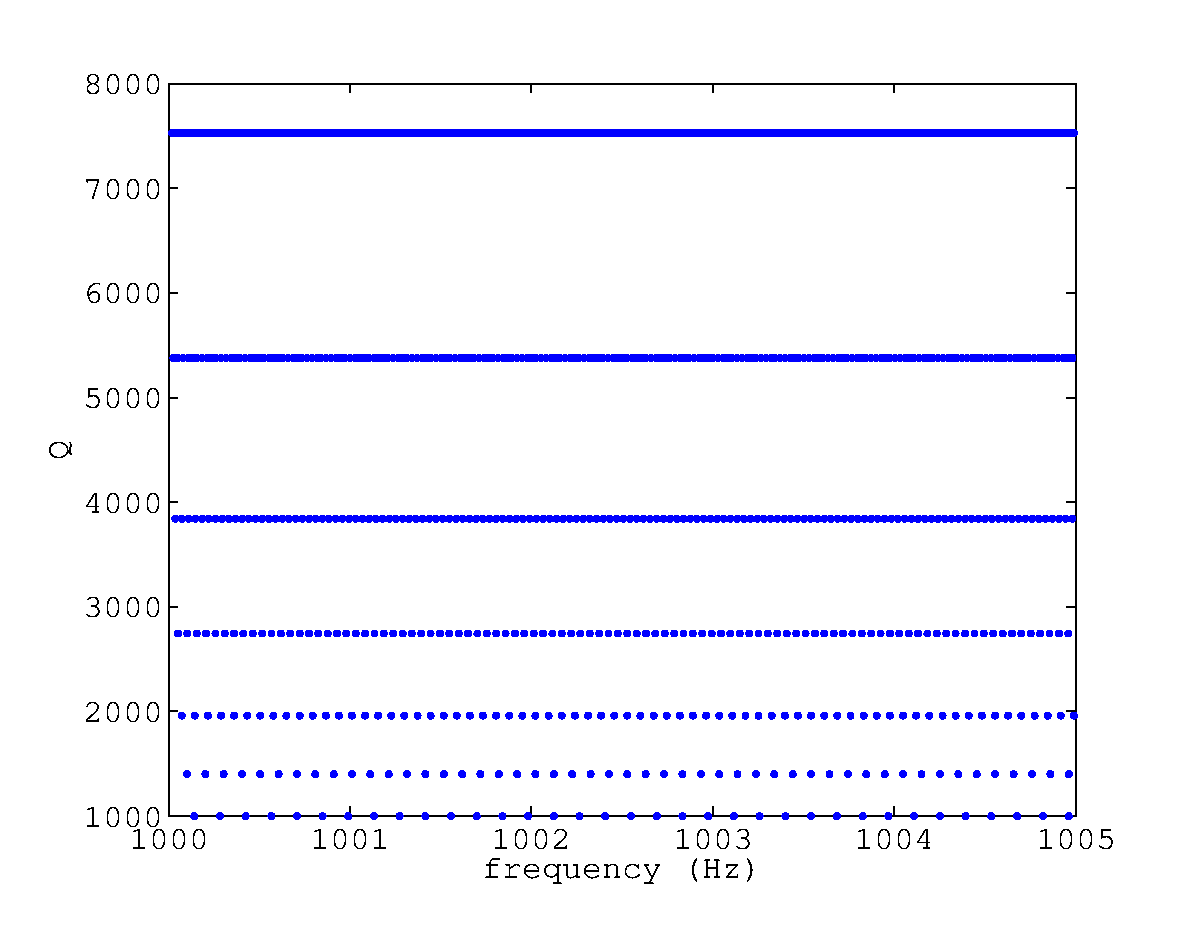
\includegraphics[width=0.6\textwidth]{figs/ringTemplates}\caption[Template bank for our ring-down
parameters $f$ and $Q$.]{Template bank for our ring-down parameters over the range $f ({\rm Hz}) =
[1000, 1005]$ and $Q = [1000, 10000]$ with a mismatch of 1\%.}\label{ringTemplates}
\end{center}
\end{figure}
It can been seen that the coverage of the $Q$ range can be quite coarse while that for $f$ is quite
fine meaning that there will still be a quite fine coverage of $\tau$.

There is obviously a trade-off between the number of templates used (which will increase for
smaller mis-matches and larger parameter ranges) and the speed of the search, so the value of the
mis-match needs to be chosen with this in mind.

Code to perform a ring-down search using matched filtering with a template bank as described
above has been developed in LALapps \cite{LALapps} in the main by Jolien Creighton. This search was
initially intended to look for black hole ring-downs after mergers as in Creighton (1999)
\cite{Creighton:1999}, where the values of $Q$ and $f$ can be used to imply parameters of the
black hole. The simple ring-down template also applies to our case of neutron star ring-downs, so we
are able to make use of the code for these purposes. 

\subsection{Bayesian evidence based search}
% show Bretthorst stuff
Bretthorst (1988) \cite{Bretthorst:1988} looks into the problem of parameter estimation for
ring-down signals in noise, with the frequency and decay time being the parameters of interest. He
derives a joint posterior probability distribution for the ring-down frequency and decay time of
\begin{equation}\label{RingPosterior}
p(f, \tau|D, I) \propto \left[1 - \frac{R(f, \tau)^2 + I(f, \tau)^2}{Nc\bar{d^2}}
\right]^{\frac{2-N}{N}},
\end{equation}
where
\begin{eqnarray}
R(f, \tau) & = & \sum_{i=1}^N d_i \cos{(2\pi{}ft_i)} e^{-t_i/\tau}, \\
I(f, \tau) & = & \sum_{i=1}^N d_i \sin{(2\pi{}ft_i)} e^{-t_i/\tau}, \\
c & \approx & \frac{1}{2}\sum_{i=1}^N e^{-2t_i/\tau},
\end{eqnarray}
and
\begin{equation}
\bar{d^2} = \frac{\sum_{i=1}^N d_i^2}{N},
\end{equation}
where $d_i$ are the data points. The ring-down amplitude and phase (see equation~\ref{Ringdown})
have been analytically marginalised over using uniform priors, as has the unknown noise standard
deviation (using a Jeffreys prior) in a similar way to that described in Chapter~2 for the pulsar
parameter estimation, leaving a Student's-t-like distribution. This posterior only holds under the
assumptions of no low frequency components in the data, i.e. $t \gg 1/f$ (as approximations are made
in averaging sinusoids to zero) and that there is a large data set, $N \gg 1$. The use of this as a
parameter estimation tool can be seen in figure~\ref{ringPosterior}, where a ring-down signal has
been injected into noise and the posterior pdf extracted using the above method.
\begin{figure}[!htbp]
\begin{center}
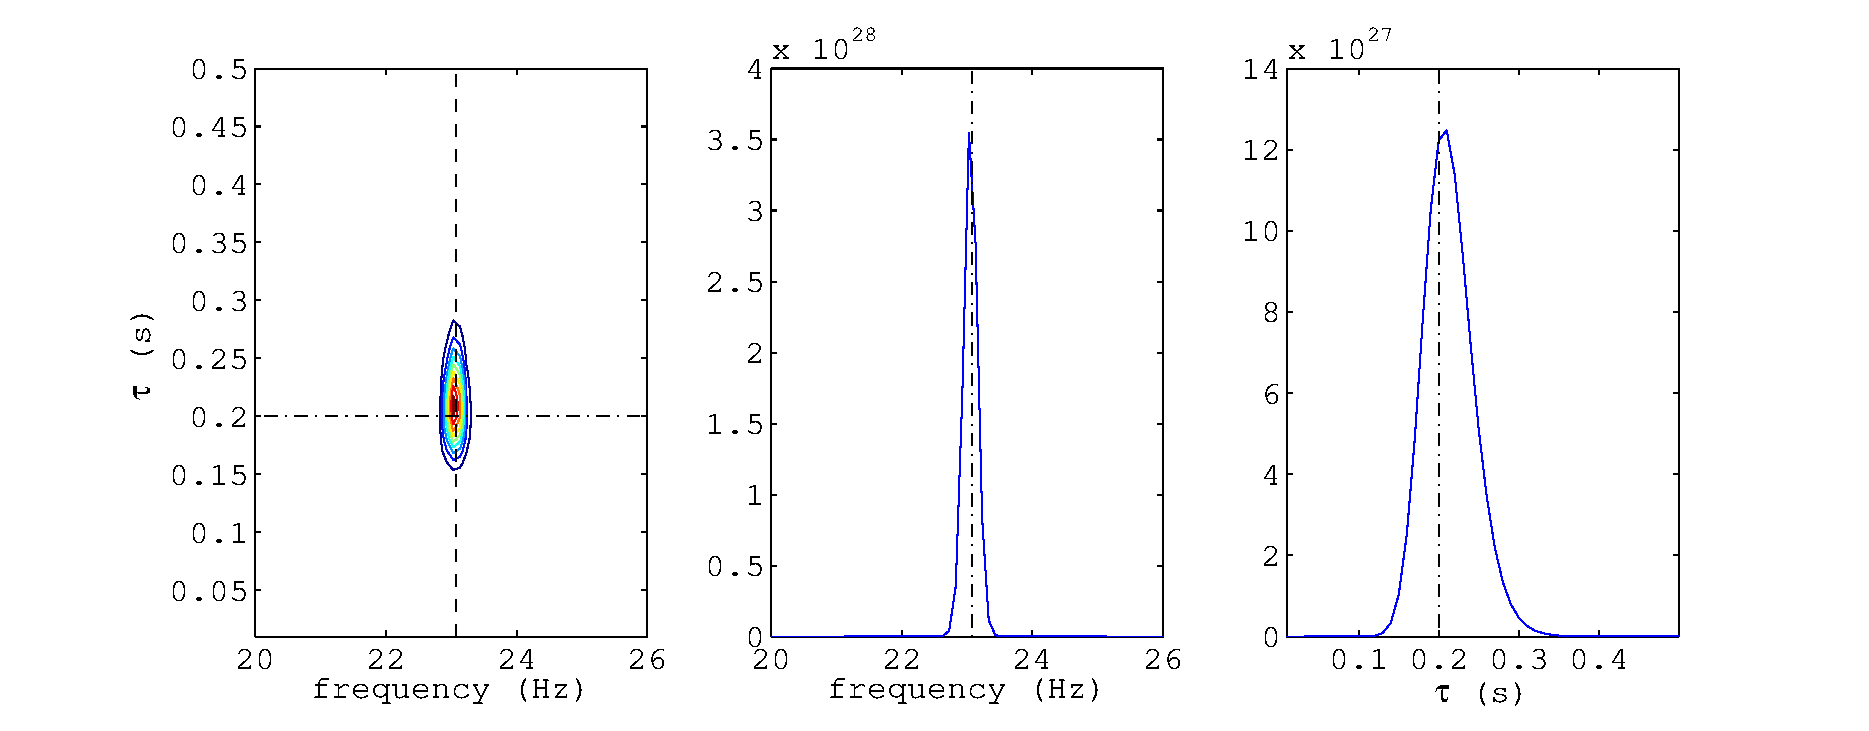
\includegraphics[width=1.0\textwidth]{figs/ringPosterior}\caption[The posterior pdfs
for the ring-down parameters $f$ and $\tau$.]{The posterior pdfs for the ring-down parameters $f$
and $\tau$. The dotted black lines represents the true signal parameters. The left-hand plot shows
the joint pdf with probability contours. The other two plots show marginalised pdfs for each
parameter.}\label{ringPosterior}
\end{center}
\end{figure}
A comparison of this method for parameter estimation of ring-down frequencies with that of more
classical Fourier power spectrum and periodogram analyses is given in \cite{Bretthorst:1988} and can
be seen in figure~\ref{BayesVsFFT}.
\begin{figure}[!htbp]
\begin{center}
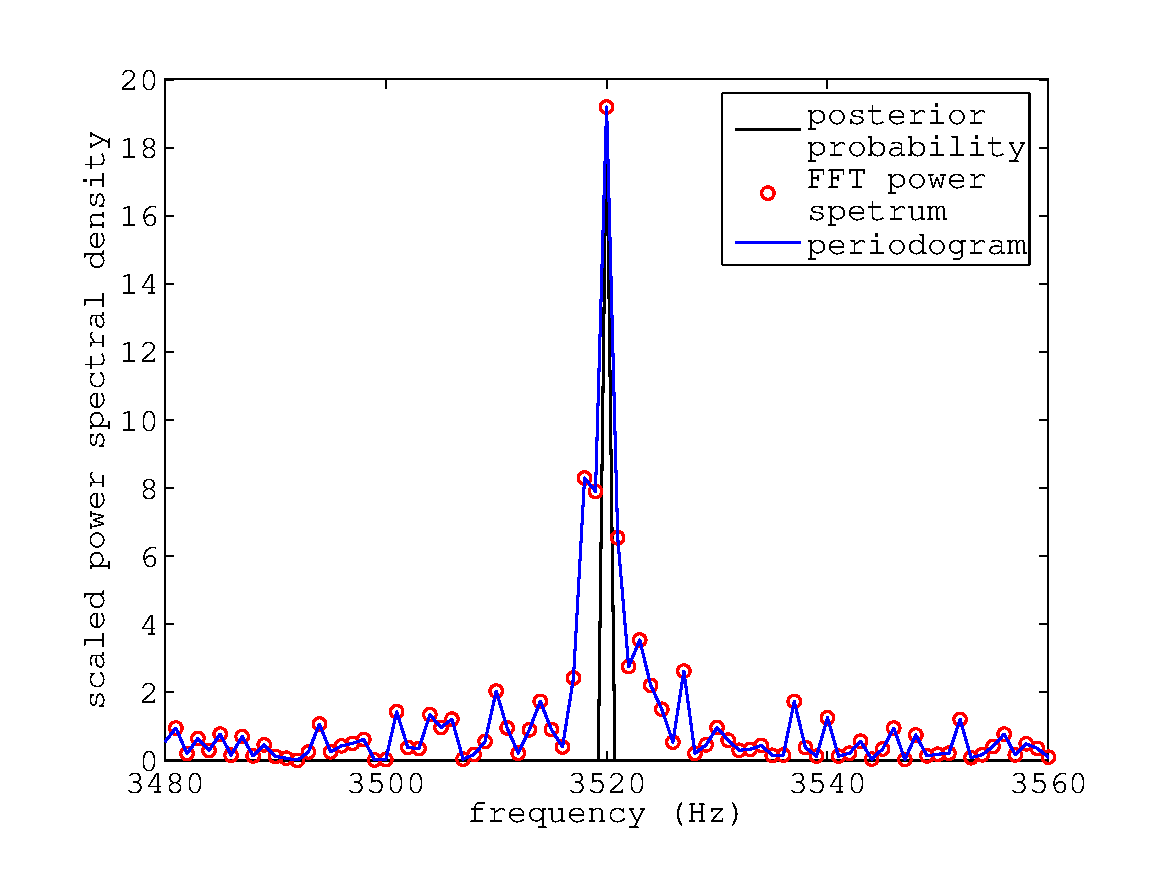
\includegraphics[width=0.6\textwidth]{figs/BayesVsFFT}\caption[A comparison of the posterior pdf,
with a periodogram and power sepctrum for a ring-down signal.]{A comparison of the posterior pdf
from equation~\ref{RingPosterior} marginalised over $\tau$, and the periodogram and power spectrum
for a ring-down signal (with amplitude = 1, $f=3519.9$\,Hz and $\tau = 0.11$\,s) injected into
Gaussian noise with $\sigma = 1$.}\label{BayesVsFFT}
\end{center}
\end{figure}
Figure~\ref{BayesVsFFT} shows how the Bayesian estimation technique can be far superior in pinning
down the parameter value over more traditional methods.

This parameter estimation can be extended into a potential search for ring-down signals in which the
parameter values are not considered important but the evidence of any signal being present is
wanted. By marginalising over the range of the frequency and decay time parameters a single value is
obtained called the evidence,
\begin{equation}
{\rm evidence} = \int_{f_{\rm min}}^{f_{\rm max}}\int_{\tau_{\rm min}}^{\tau_{\rm max}} p(f,
\tau|I)p(D|f,\tau,I) {\rm d}f{\rm d}\tau, 
\end{equation}
which tells us something about the presence or absence of any ring-down signals in the given range.
To evaluate its efficacy some comparison is needed between the value of the evidence when only noise
is present to that when a ring-down signal is present. 

To get an idea of how this algorithm performs when a signal is not present we have performed
extensive simulations on 1000 realisations of Gaussian noise. This used a uniformly placed
$4001\times21$ grid in $f({\rm Hz}) = [1000, 4000]$ and $\tau(s) = [0.05, 0.5]$ to evaluate
the posterior and perform the marginalisation, where the grid size was chosen as the best
compromise between computational speed and parameter extraction accuracy from many trial grids. A
plot of the evidence values obtained can be seen in figure~\ref{evidenceNoise}. This has a mean
value of $\log{\rm evidence} = 5.97$ and shows $\log{\rm evidence}$ values extending to $\sim 8.5$.
\begin{figure}[!htbp]
\begin{center}
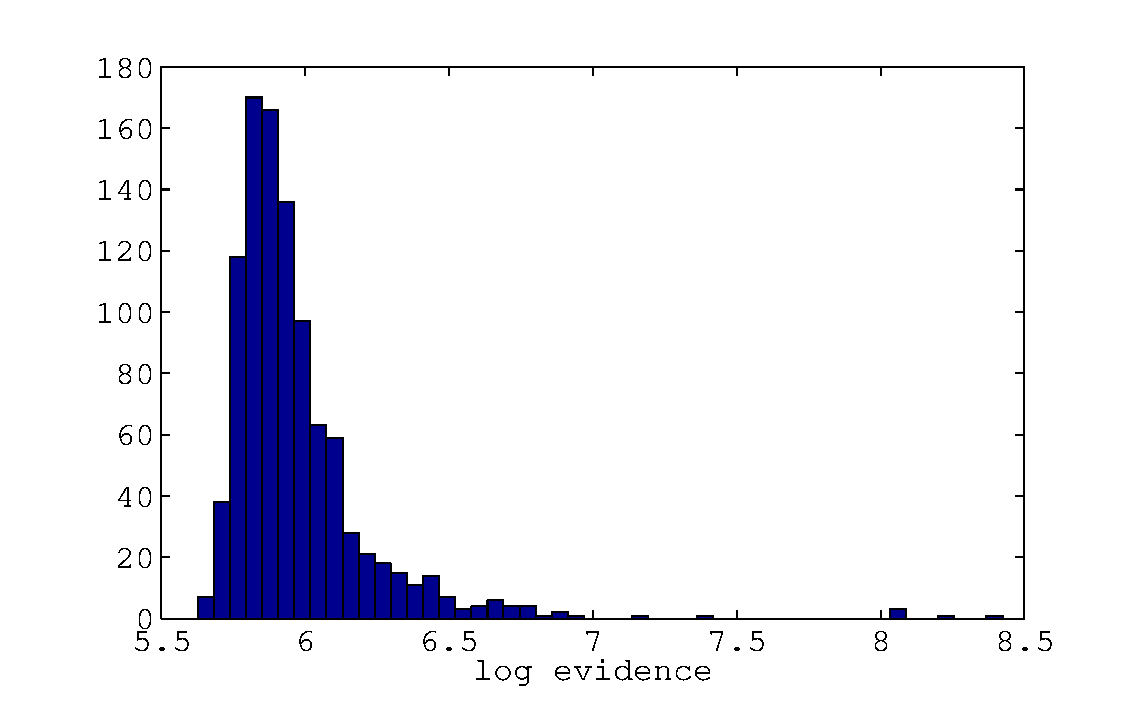
\includegraphics[width=0.6\textwidth]{figs/evidenceNoise}\caption[Evidence of a ring-down
signal in Gaussian noise.]{Evidence of a ring-down signal in 1000 independently realised one second
(sampled at 16384\,Hz) sets of Gaussian noise.}\label{evidenceNoise}
\end{center}
\end{figure}

\section{Ring-down search from 27$^{\rm th}$ December 2004 $\gamma$-ray burst of SGR\,1806-20}
\subsection{Soft $\gamma$-ray Repeaters}
Soft $\gamma$-ray repeaters (SGRs) are seen as sources of short, extremely high luminosity bursts of
soft spectrum $\gamma$-rays. Their periods of burst activity can be sporadic with extremely active
periods followed by lengthy quiet periods. SGRs are also seen as quiescent soft X-ray sources.
There are currently four (possibly five) SGRs known, a review of which can be found in Hurley (2000)
\cite{Hurley:2000}. The collocation of SGRs with supernova remnants has lead to the hypothesis that
they are a class of very highly magnetised neutron stars called magnetars. Such stars have
dipole magnetic fields of $B \sim 10^{14}-10^{15}$\,G (cf. $\sim 10^{12}$\,G for normal pulsars and
$\sim 10^8$\,G for millisecond pulsars), which means they will quickly spin-down via magnetic
breaking.

SGRs are occasionally seen to emit giant flares of $\gamma$-rays, with thousands of times the
luminosity of ordinary bursts and with harder spectra. The identification of these short duration
($\sim 0.2$\,second) $\gamma$-ray bursts (GRBs) with SGRs provides a possible source of some
classical GRBs without any known counterpart. The cause of such giant bursts is discussed in Hurley
{\it et al.} (2005) \cite{Hurley:2005} and is thought to be a result of some extreme instability in
the magnetar involving crustal breaking and magnetic reconnection, with huge amounts of energy
coming from the untwisting of the magnetosphere. Such reconfigurations of the crust and magnetic
field could set up oscillations in the star (see Ioka, 2001 \cite{Ioka:2001} and Kokkotas and
Schmidt, 1999 \cite{Kokkotas:1999}) which will be damped by emission of gravitational waves. This
makes giant flares from SGRs a potential target for our ring-down search. Various methods of energy
release to power the flares and possible \gw emission are discussed in Horvath (2005)
\cite{Horvath:2005}.

On 27$^{\rm th}$ December 2004 the most luminous SGR flare yet seen was observed from SGR\,1806-20
\cite{Hurley:2005}. It was observed by five separate space-based $\gamma$-ray detectors and such was
its intensity that it briefly saturated them all. The flare lasted $\sim 380$\,seconds with an
initial 0.2\,second spike. The event information is shown in table~\ref{SGR1806-20Burst}.
\begin{table}[!htbp]
\caption{\label{SGR1806-20Burst} The parameters of SGR\,1806-20 and the giant flare.}
\begin{center}
\begin{tabular}{| l | l |}
\hline
\multicolumn{2}{| c |}{SGR\,1806-20} \\
\hline \hline
$\alpha$ & $15^{\rm h}56^{\rm m}37^{\rm s}$ \\
$\delta$ & $-20^{\circ}$13'50'' \\
Distance & $\sim 15$\,kpc \\
Burst time & 21:30:27 UTC 27-Dec-2004 \\
Burst duration & 200\,ms \\
\hline
\end{tabular}
\end{center}
\end{table}
Although the time of this burst was outside of any LSC science run period, both the LIGO H1 detector
and \geo were taking data at the time. This gives the interesting possibility of performing a
targeted search for \gws from this source.

A search for \gws from quasi-normal modes of this source has already been performed using data from
the AURIGA bar detector (see Baggio {\it et al.}, 2005 \cite{Baggio:2005}). It had a limited
bandwidth of $\sim 100$\,Hz around their detectors most sensitive frequency of 900\,Hz (below the
expected $f$-mode frequency range). This search performed a time convolution of the data with the
ring-down signal model for 10\,s around the peak of the burst over a range of $f$ values spaced at
$\Delta{}f = 1/(2\tau) = 5$\,Hz, where $\tau = 100$\,ms, and with time steps $\Delta{}t =
201.5$\,ms. This method did not make use of optimal matched filtering. This gave an upper limit
across the frequency range on the total \gw energy of around $10^{-5}\,{\rm M}_{\odot}c^2$.

We can obtain an upper limit estimate on the \gw amplitude from this burst using the equations in
\S\ref{sec:ringdownsignal}. In Woods {\it et al.} (2005) \cite{Woods:2005} an upper limit on the
change in frequency of SGR\,1806-20 during the GRB is given as $\Delta{}f < 2\ee{-5}$\,Hz. Taking
this value and assuming the model of angular momentum exchange between interior and crust we can get
an upper limit on the energy release of $\Delta{}E < 10^{34}-10^{36}$\,J (for the range of
$\Omega_{\rm lag}$), which is very similar to that for large glitches of the Vela pulsar. With a
distance to SGR\,1806-20 of $\sim 15$\,kpc, and again assuming all the energy goes into exciting
$f$-modes and using equation~\ref{RingAmplitude} we get an upper limit range of $h_{\rm eff} <
10^{-23}-10^{-24}$. From the discussion in \cite{Hurley:2005} breaking of the crust, and therefore a
change in the moment of inertia, seems a more likely mechanism of energy release to set up stellar
oscillations. With a period of 7.48\,s an upper limit on the relative change in moment of inertia
can be calculated giving an energy release of $\Delta{}E < 10^{35}$\,J and a \gw amplitude upper
limit on $h_{\rm eff} < 5\ee{-24}$. These energies are still orders of magnitude less than that
given off in $\gamma$-rays at the peak of the flare with $E \approx 3.5\ee{39}$\,J
\cite{Hurley:2005}. The energy for which can be explained by the release of energy stored in the
twisted magnetic field ($E_{\rm twist} \sim 10^{39}$\,J) via magnetic reconnection. 

\subsection{A preliminary search}

\subsubsection{First look}
The first thing we did upon receiving information about the $27^{\rm th}$ December 2004 GRB was to
look by eye at the data for any obvious signal. The data from 20\,s around the time of the burst,
high-pass filtered at 900\,Hz, are shown as a time series in figure~\ref{SGRTimeSeries} and a
spectrogram in figure~\ref{SGRSpecgram}.
\begin{figure}[!htbp]
\begin{center}
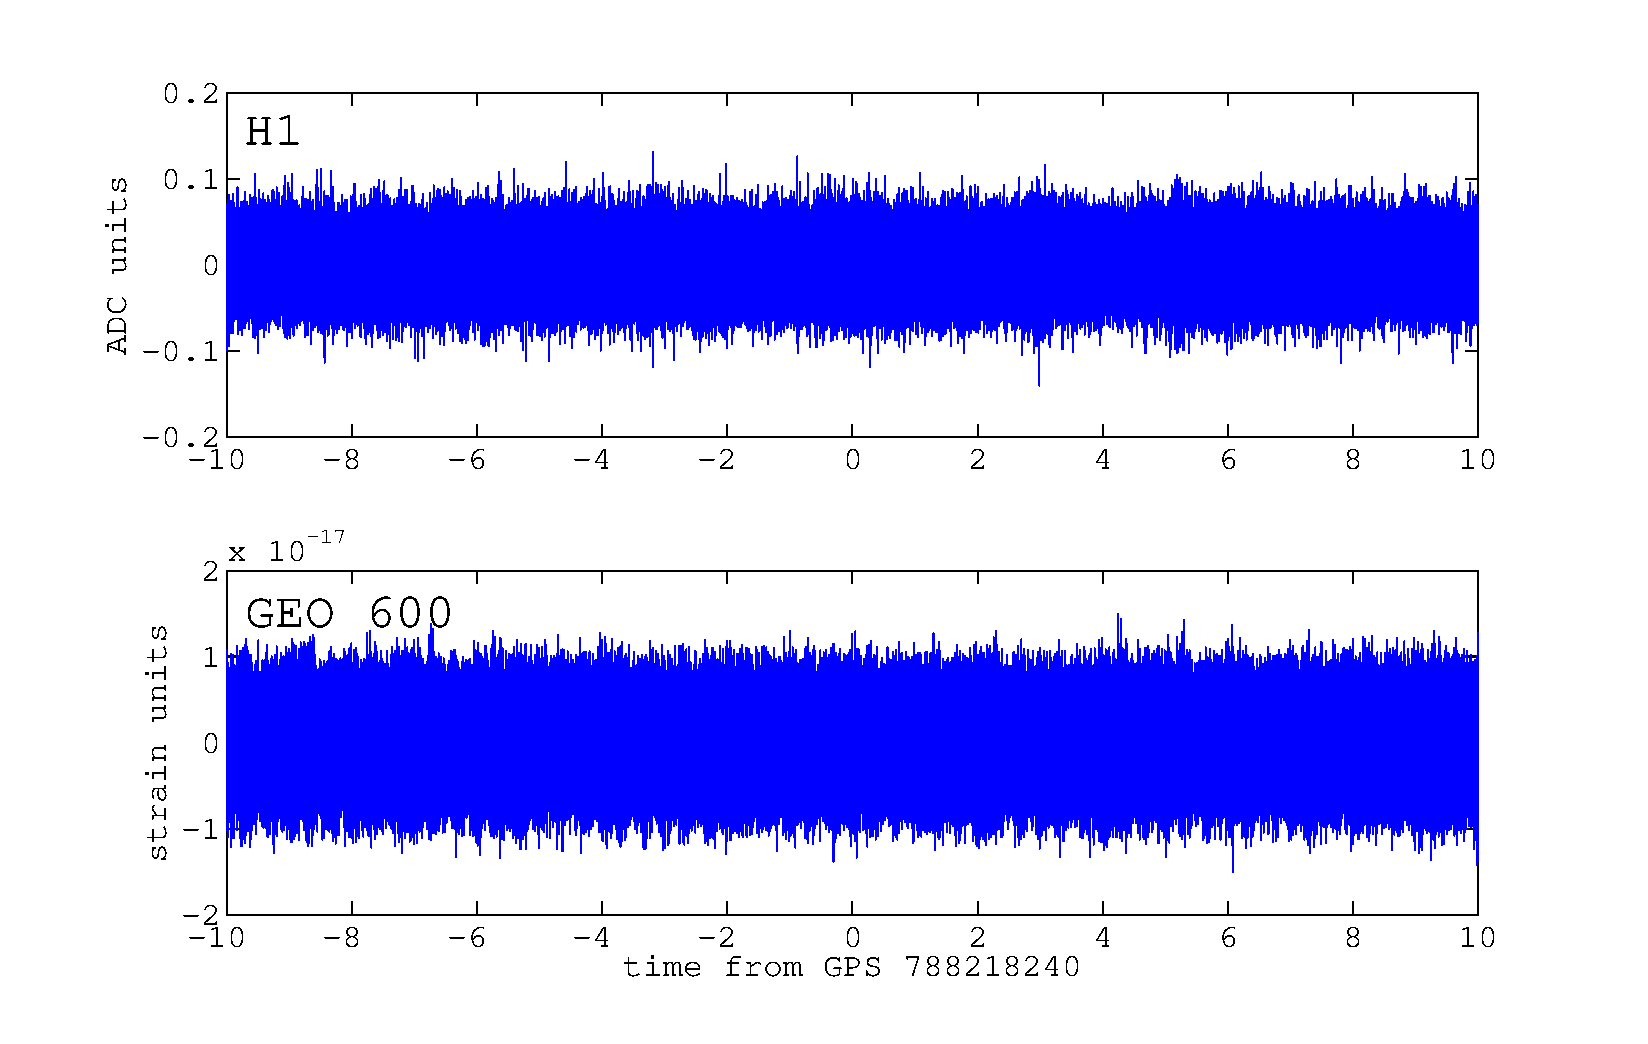
\includegraphics[width=1.0\textwidth]{figs/SGRTimeSeries}\caption[The time series of data from H1
and \geo for 20 seconds around the time of the $27^{\rm th}$ December 2004 GRB.]{The time series of
data from H1 and \geo for 20 seconds around the time of the $27^{\rm th}$ December 2004 GRB. The
data has been high-pass filtered at 900\,Hz with an $8^{\rm th}$ order Butterworth
filter.}\label{SGRTimeSeries}
\end{center}
\end{figure}
\begin{figure}[!htbp]
\begin{center}
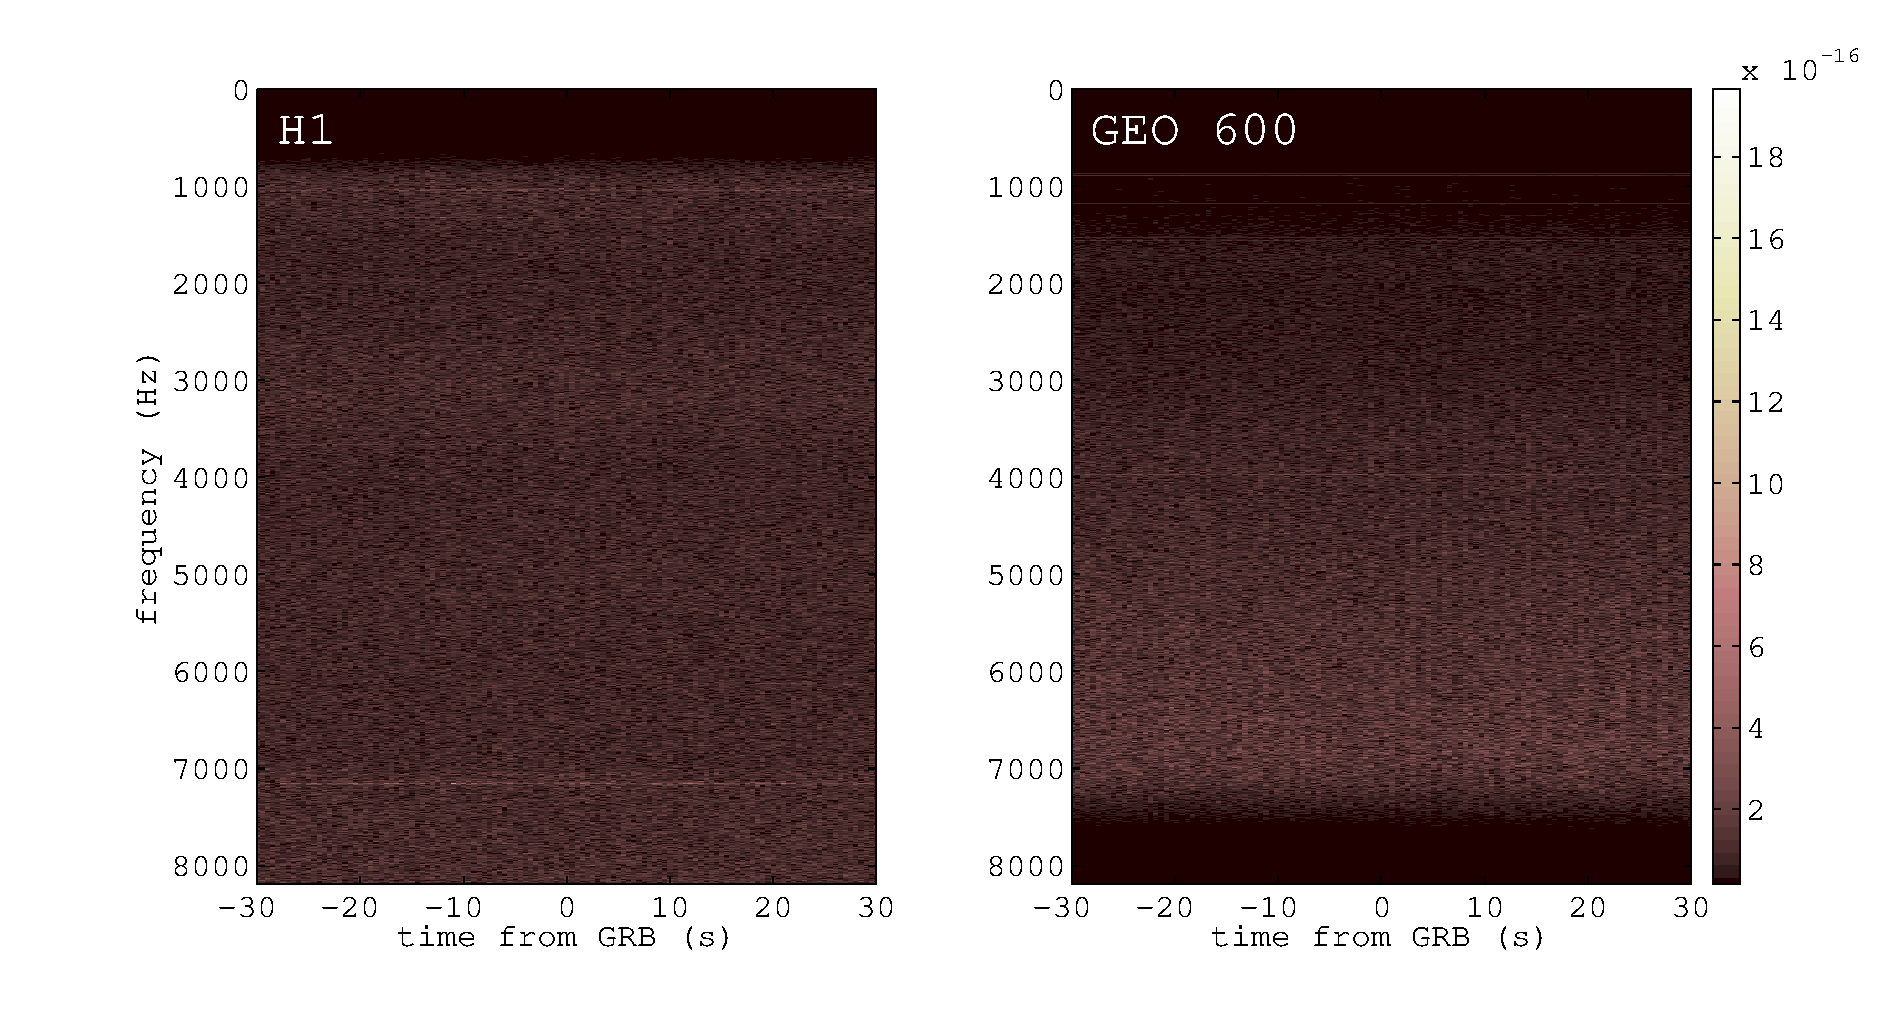
\includegraphics[width=1.0\textwidth]{figs/SGRSpecgram}\caption[The spectrogram of data from H1 and
\geo for 60 seconds around the time of the $27^{\rm th}$ December 2004 GRB.]{The spectrogram of
data from H1 and \geo for 60 seconds around the time of the $27^{\rm th}$ December 2004 GRB. The
data has been high-pass filtered at 900\,Hz with an $8^{\rm th}$ order Butterworth filter and the
strength of the \geo calibration lines has been suppressed for contrast.}\label{SGRSpecgram}
\end{center}
\end{figure}
No obvious glitch is seen in this data above the level of the noise floor.

Szabolcs Marka and Peter Kalmus \cite{Szabi} have also been looking at this data for a possible low
frequency burst, but for our quasi-normal mode search the low frequencies have been filtered out.
In the low frequency region the \geo data does not really help as its sensitivity below $\sim
1000$\,Hz is much worse than H1.

\subsubsection{Matched filter search}
After the initial examination of the data we have made use of the LALapps ring-down code (as
described in \S\ref{matchedfiltering}) to search for signals in the data at the time of the GRB.
This work was performed with the help of an undergraduate summer student Edward Bloomer as part of
a {\it Robert Cormack Bequest Scholarship}. The ring-down code takes in several parameters to
perform the search which have been chosen with our particular targets in mind. These were: $f ({\rm
 Hz}) = [1000, 4000]$, $Q = [1000, 10\,000]$, $\phi_0 = 0$, high-pass frequency = 800\,Hz, and a
maximum template mismatch of 10\%. This produces a template bank of $26\,023$ filters spaced as is
shown in figure~\ref{SGRTemplateBank}. 
\begin{figure}[!htbp]
\begin{center}
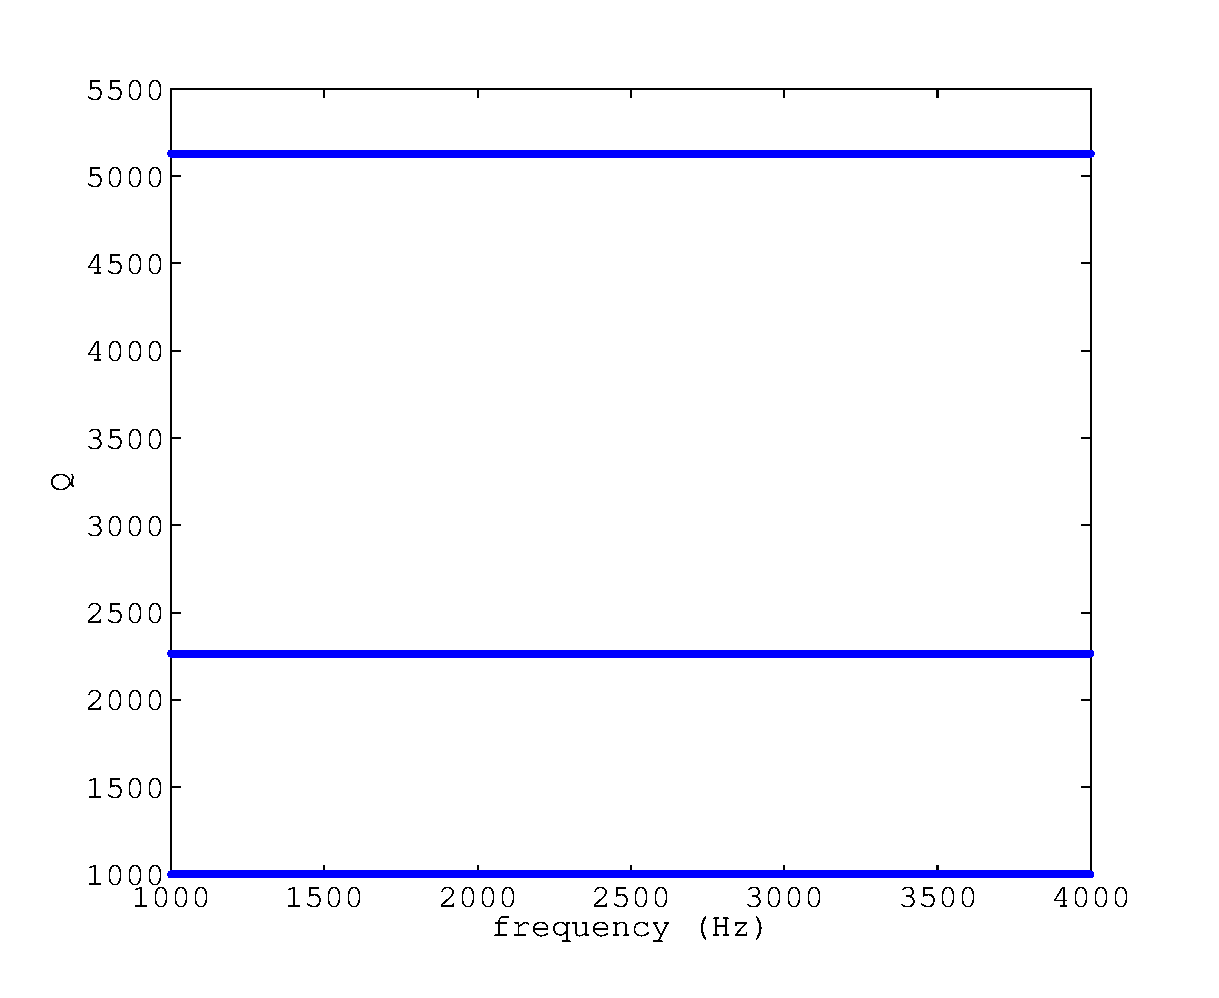
\includegraphics[width=0.6\textwidth]{figs/SGRTemplateBank}\caption{The template bank
for the ring-down search with $f ({\rm Hz}) = [1000, 4000]$, $Q = [1000, 10\,000]$, and a maximum
mismatch of 10\%.}\label{SGRTemplateBank}
\end{center}
\end{figure}
The code will then output triggers if any of the templates match the data above a certain $S/N$
threshold. The level of this threshold needs to be set carefully as even Gaussian noise will
give a underlying level of template matching. To determine the threshold to use for our data around
the time of the GRB, we ran the code on simulated data and data from periods off-source, giving
us a background level. Running the code over 120 seconds of simulated Gaussian noise (using the low
$S/N$ threshold of 1), gives us an idea of the background distribution of events picked up by the
matched filtering (see figure~\ref{RingSimDataHist}).
\begin{figure}[!htbp]
\begin{center}
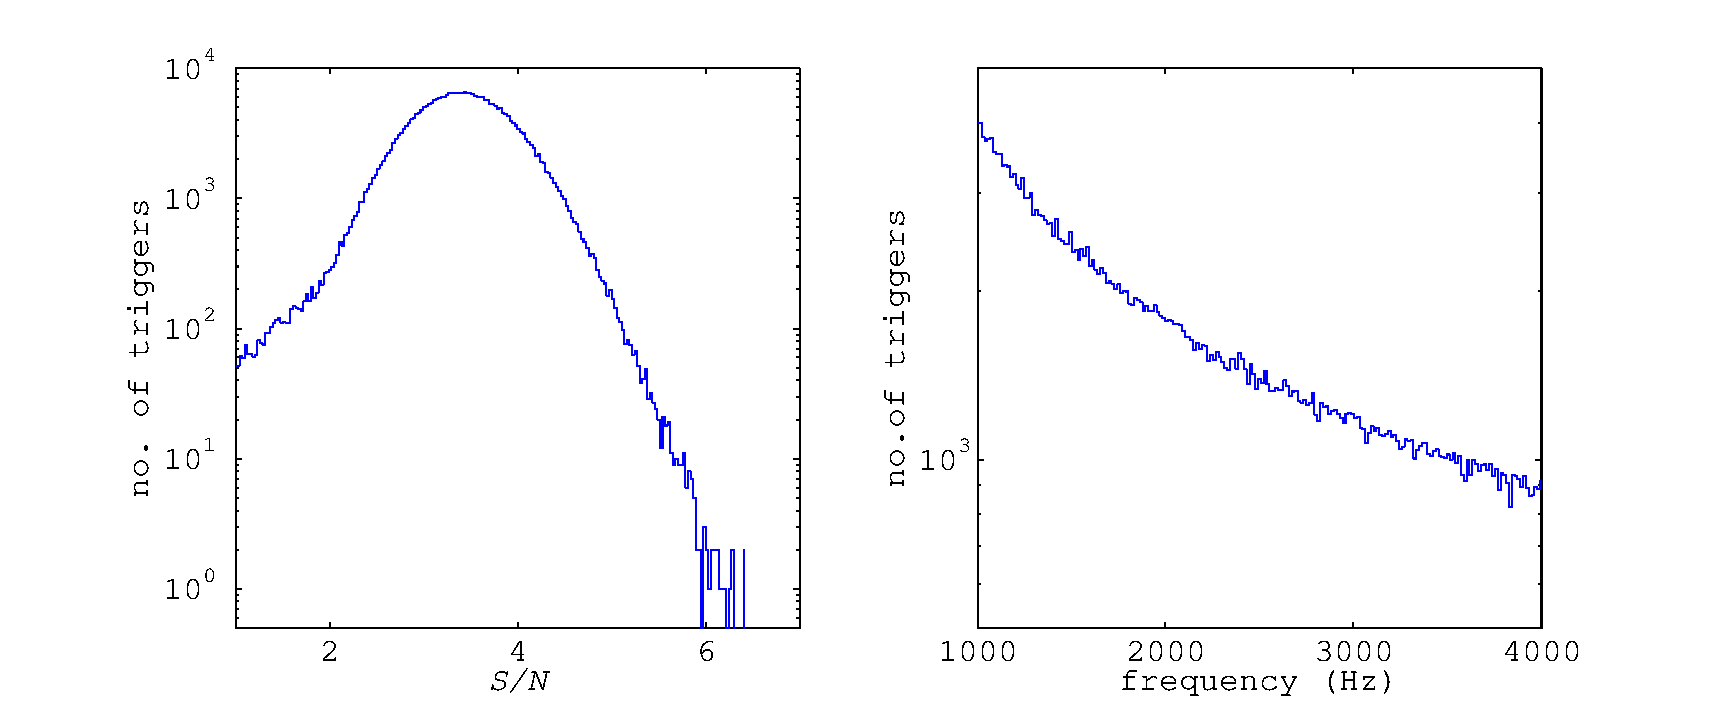
\includegraphics[width=1.0\textwidth]{figs/RingSimDataHist}\caption{The number of triggers at given
$S/N$ and frequency for the LALapps ring-down code using 120 seconds of Gaussian
noise.}\label{RingSimDataHist}
\end{center}
\end{figure}
It can be seen from figure~\ref{RingSimDataHist} that there is a clustering of events around an
$S/N$ of 3, with a tail extending out to $\sim 7$. This shows that even in completely Gaussian noise
the code gives a background of events and a threshold of $S/N$ $> 7$ is probably needed unless the
events can be vetoed in some other way.

Simulated white noise does not necessarily reflect the true nature of our data which can contain
many artifacts, either continuous, like instrumental lines, or transient in nature. The same search
was therefore performed (using the parameters given above for the simulated noise) on 120\,s of data
approximately half an hour after the GRB. Here the threshold has been increased to an $S/N$ of 5 to
avoid the large number of events around $S/N \approx 3$. For H1 the data is uncalibrated and
whitened, and as the calibration lines lie below 1000\,Hz they are out of our band
\cite{CalibrationDoc}, meaning that many spectral features will be suppressed (see
figure~\ref{H1SpectrumRingdownSearch}).
\begin{figure}[!htbp]
\begin{center}
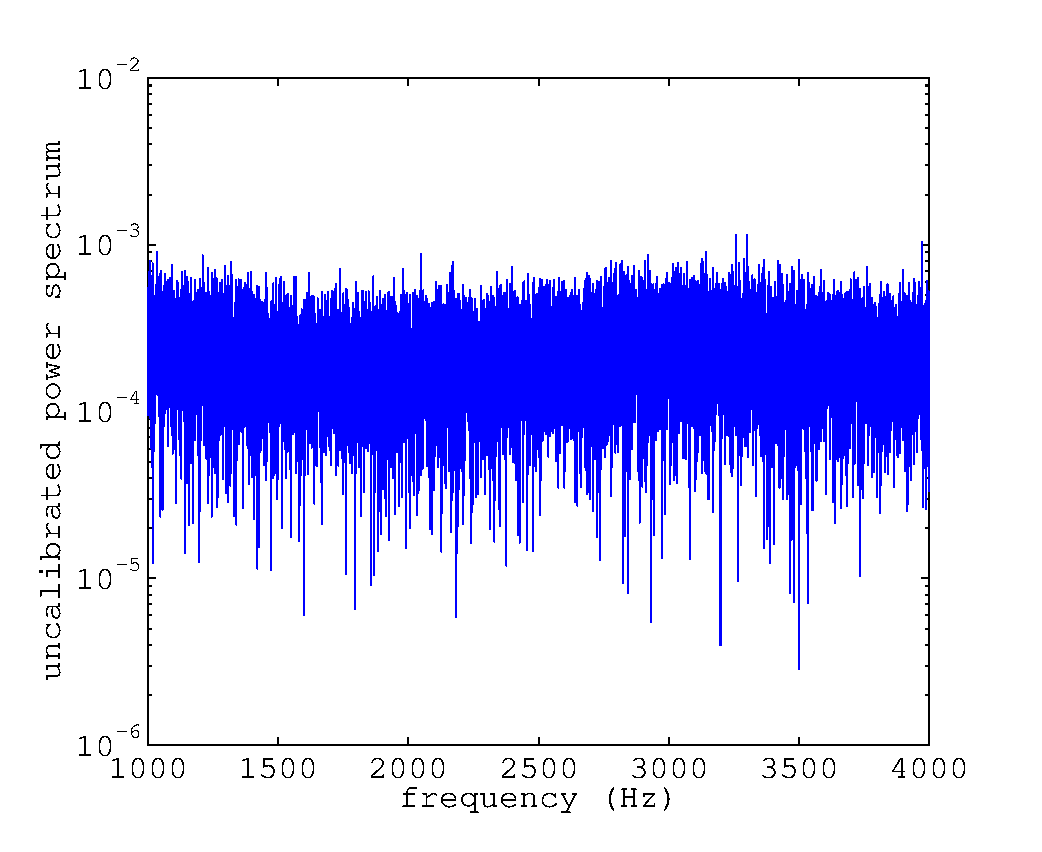
\includegraphics[width=0.6\textwidth]{figs/H1SpectrumRingdownSearch}\caption[The uncalibrated
spectrum of H1 (in ADC units) for 60\,s from GPS 78822000.]{The uncalibrated spectrum of H1 (in ADC
units) for 60\,s from GPS 78822000, high-pass filtered at 800\,Hz.}\label{H1SpectrumRingdownSearch}
\end{center}
\end{figure}
This {\it background} analysis produced a total of 2814 events with $S/N$ $> 5$ with a maximum $S/N$
of 7.2 (see figure~\ref{H1RingdownBgSNR}).
\begin{figure}[!htbp]
\begin{center}
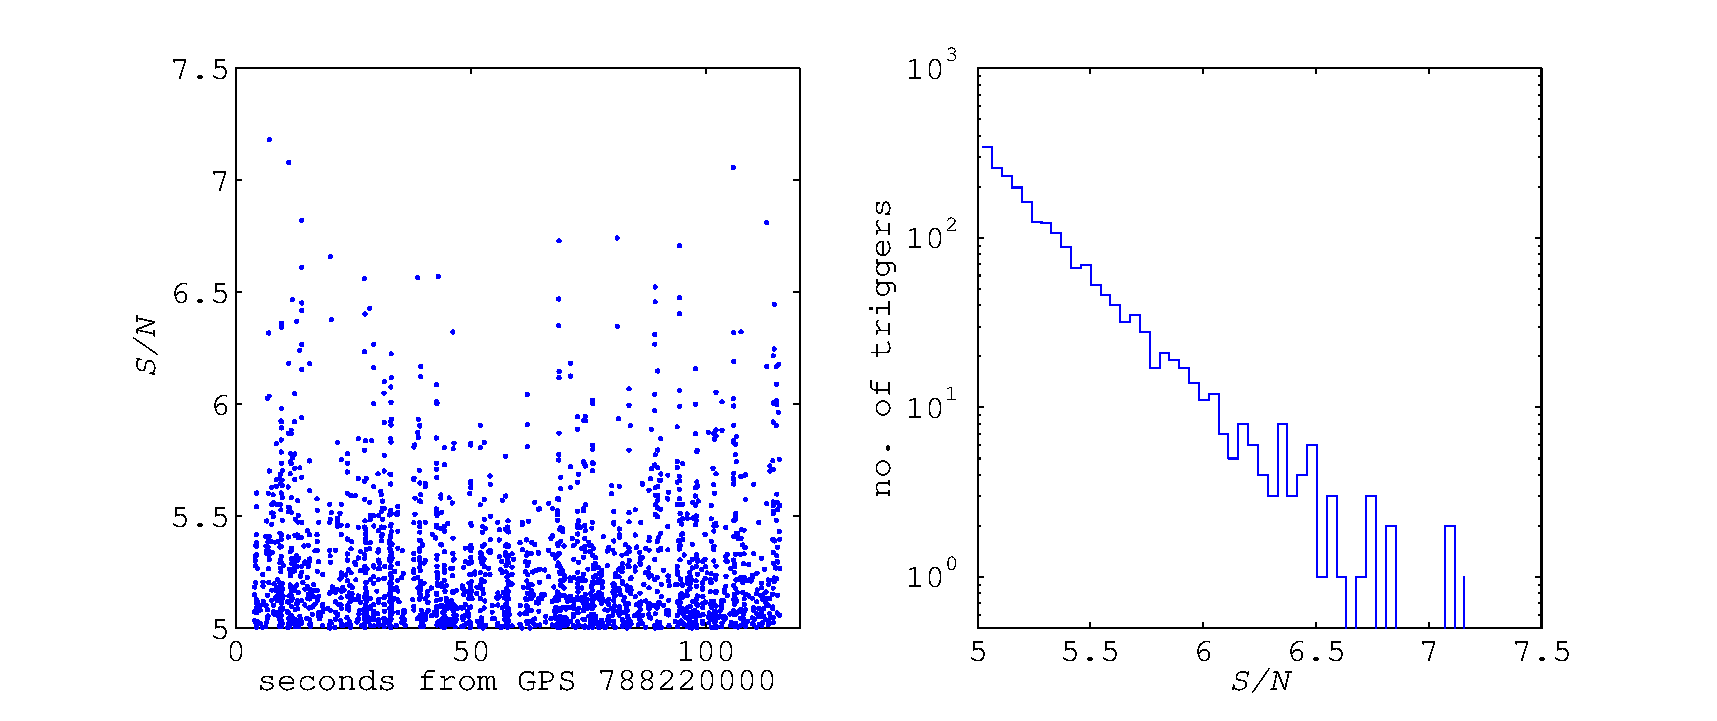
\includegraphics[width=0.8\textwidth]{figs/H1RingdownBgSNR}\caption{The distribution
in $S/N$ of events from the matched filtering algorithm for 120\,s of H1 data from GPS 788220000.
}\label{H1RingdownBgSNR}
\end{center}
\end{figure}
This is at a similar level to the analysis on Gaussian noise. The ring-down code is sensitive to
lines in the spectrum, with lines at $\sim 1040$\,Hz producing an excess of events as well as the
strongest events (see figure~\ref{H1RingdownBgFreq}).
\begin{figure}[!htbp]
\begin{center}
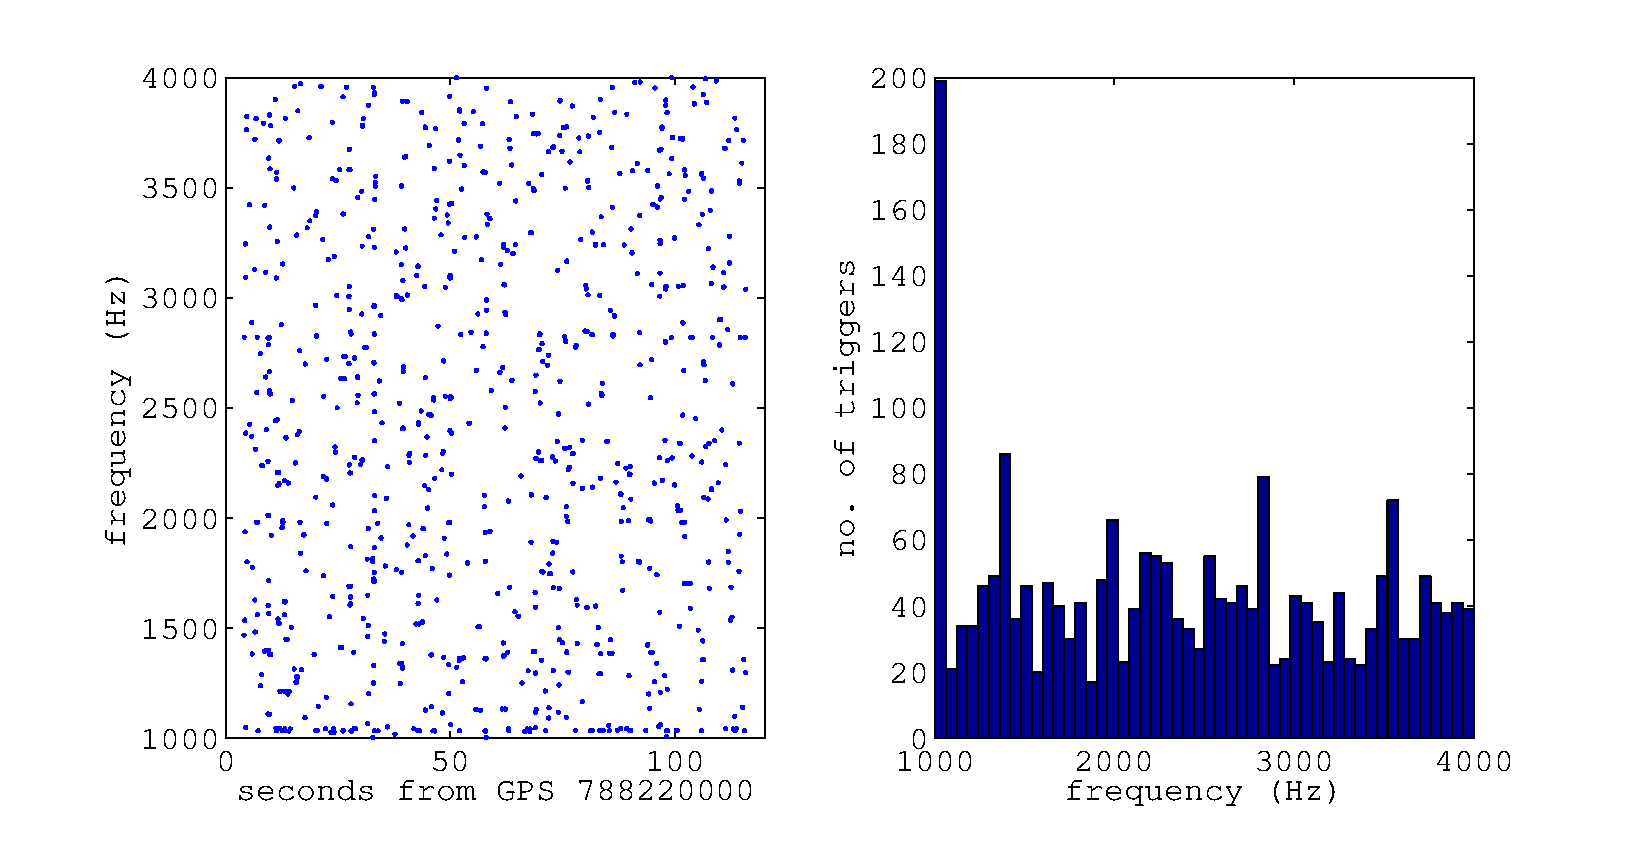
\includegraphics[width=0.8\textwidth]{figs/H1RingdownBgFreq}\caption{The distribution
in frequency of events from the matched filtering algorithm for 120\,s of H1 data from GPS
788220000.}\label{H1RingdownBgFreq}
\end{center}
\end{figure}
As certain events are from a known origin, i.e. the line, it is perhaps possible to veto them and
therefore bring down our final choice of $S/N$ cut for the results. A histogram comparing the $S/N$
of events with those thought to be caused by the line feature (between 1025-1050\,Hz) removed over
the histogram of all events is shown in figure~\ref{H1RingdownBgSNRNoLine}. It can be seen that the
strongest events ($S/N$ $> 7$) appear to be caused by the line feature, and with these removed the
maximum $S/N$ is 6.8. The fact that the line has been removed in post-processing (rather than
attempting to filter it out in the data before analysis) means that it is impossible to tell if the
events were really triggered by the line or not, so it is safest to use all the triggers for our
$S/N$ threshold rather than removing them in a semi-ad-hoc way. Figure~\ref{H1RingdownBgSNRNoLine}
also shows that, other than the obvious line-like features, the $S/N$ is fairly level across the
frequency range, meaning that it is probably best to use a single $S/N$ threshold cut across all
frequencies.
\begin{figure}[!htbp]
\begin{center}
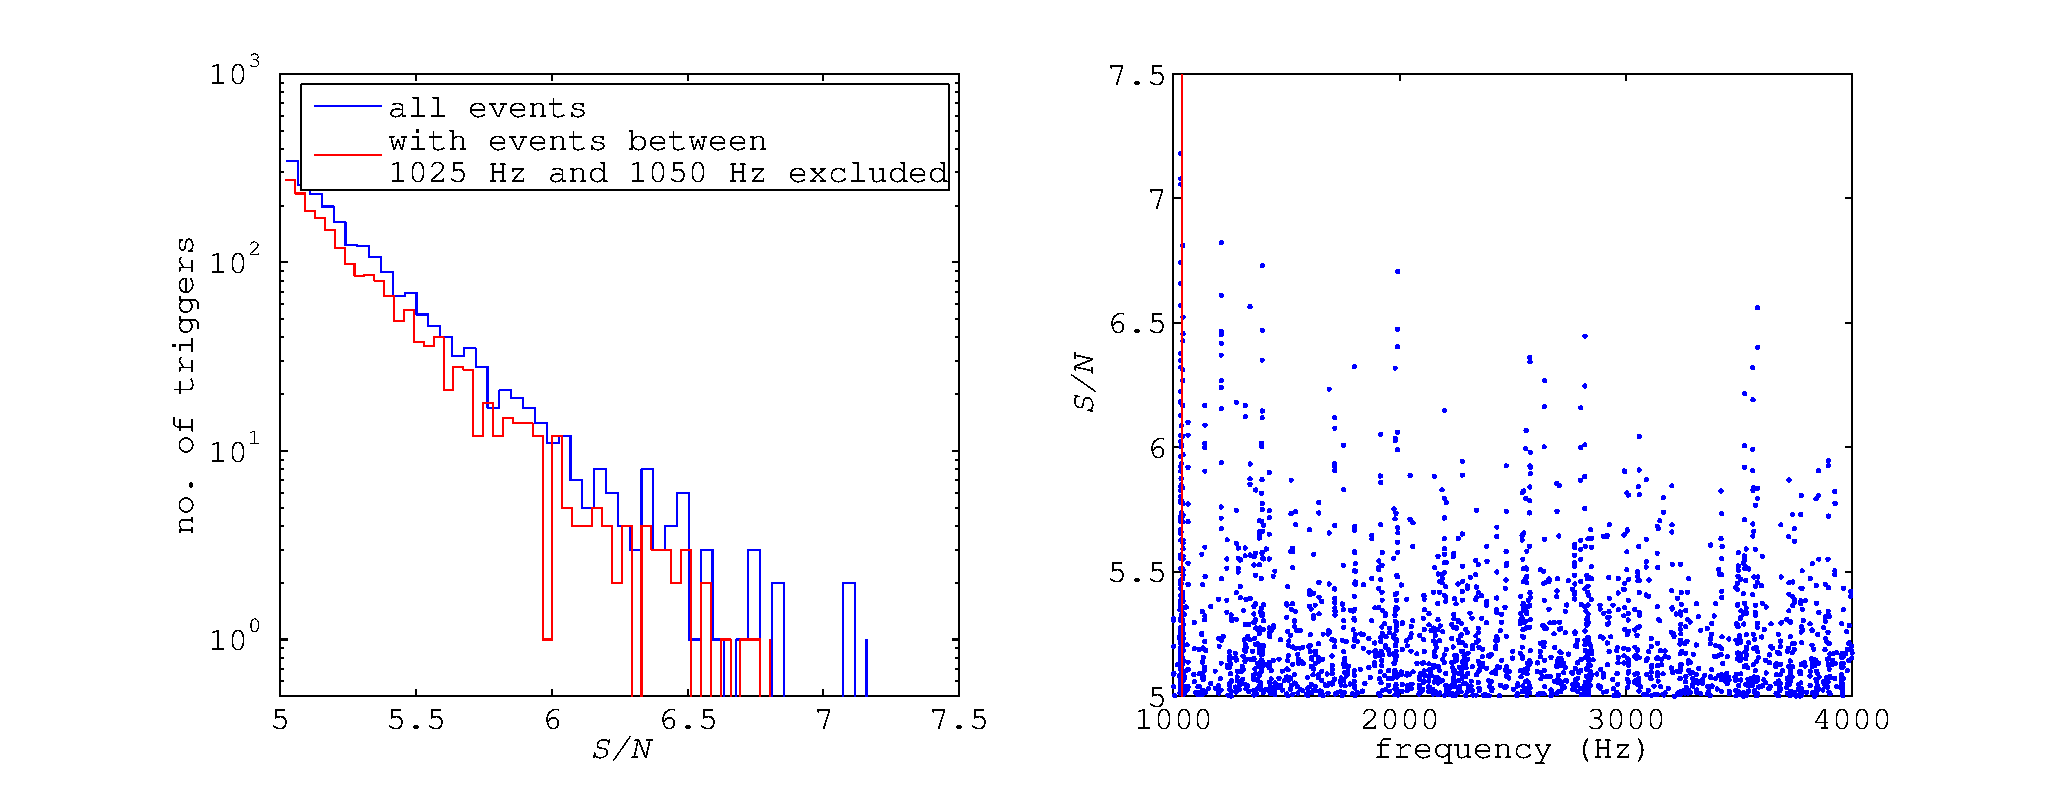
\includegraphics[width=0.9\textwidth]{figs/H1RingdownBgSNRNoLine}
\caption[A histogram of $S/n$ for events with and without certain frequencies removed.]{On the left
is a histogram of $S/N$ for events with and without removing those between the frequencies of
1025-1050\,Hz. On the right is the $S/N$ against frequency where the excess events around the $\sim
1040$\,Hz lines can be seen.}\label{H1RingdownBgSNRNoLine}
\end{center}
\end{figure}
It can been seen in figure~\ref{H1RingdownBgAmp} that there are three distinct amplitude bands of
events, which relate to the three bands of templates over $Q$ seen in figure~\ref{SGRTemplateBank}.
The band of events with the smallest amplitude relate to those with the largest $Q$ values, with
successively smaller $Q$s giving successively larger amplitude events. 
\begin{figure}[!htbp]
\begin{center}
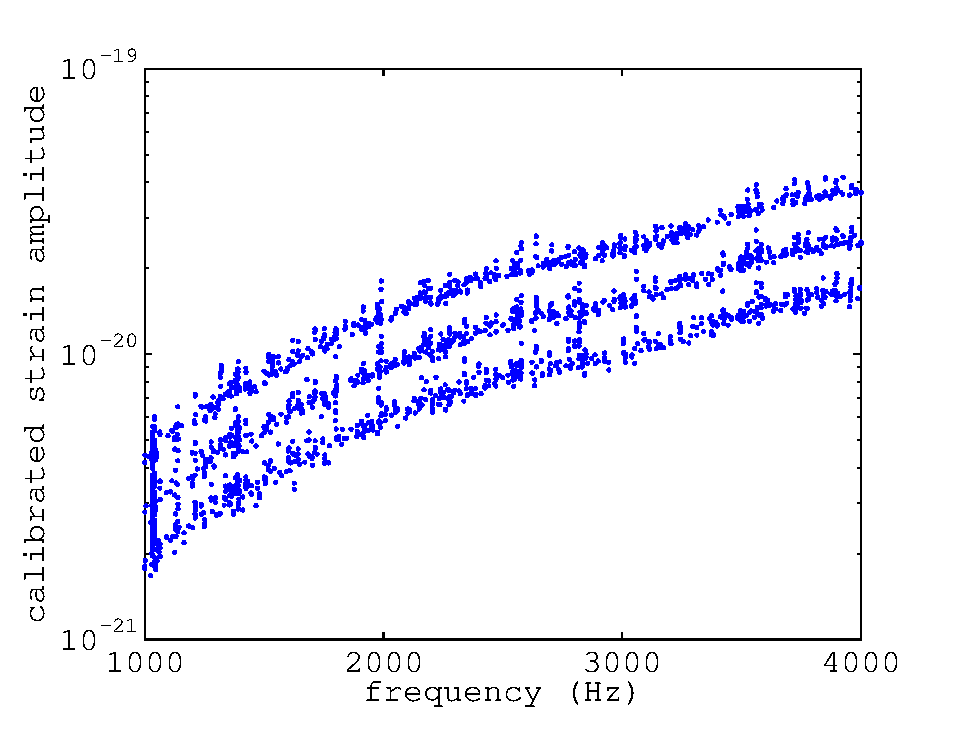
\includegraphics[width=0.6\textwidth]{figs/H1RingdownBgAmp}\caption{The calibrated
strain amplitude of events against frequency for 120\,s of H1 data from GPS
788220000.}\label{H1RingdownBgAmp}
\end{center}
\end{figure}

The \geo data being used is already calibrated and contains many large spectral features within our
search band which dominate the spectrum (see figure~\ref{GEOSpectrumRingdownSearch}).
\begin{figure}[!htbp]
\begin{center}
\includegraphics[width=0.6\textwidth]{figs/GEOSpectrumRingdownSearch}\caption[The noise spectral
density for \geo from GPS 788220060.]{The noise spectral density for \geo estimated from ten 4\,s
Hanning windowed segments with 50\% overlap from GPS 788220060.}\label{GEOSpectrumRingdownSearch}
\end{center}
\end{figure}
Again the matched filtering code was run over a 120\,s section of data away from the GRB time to
gauge a background level of events and their $S/N$s. This produced 13\,589 events with an $S/N > 5$
(see figure~\ref{GEORingdownBgSNR}), compared with the 2814 found in the H1 data, suggesting that
the \geo data is far less clean, as can indeed be seen from the spectrum.
\begin{figure}[!htbp]
\begin{center}
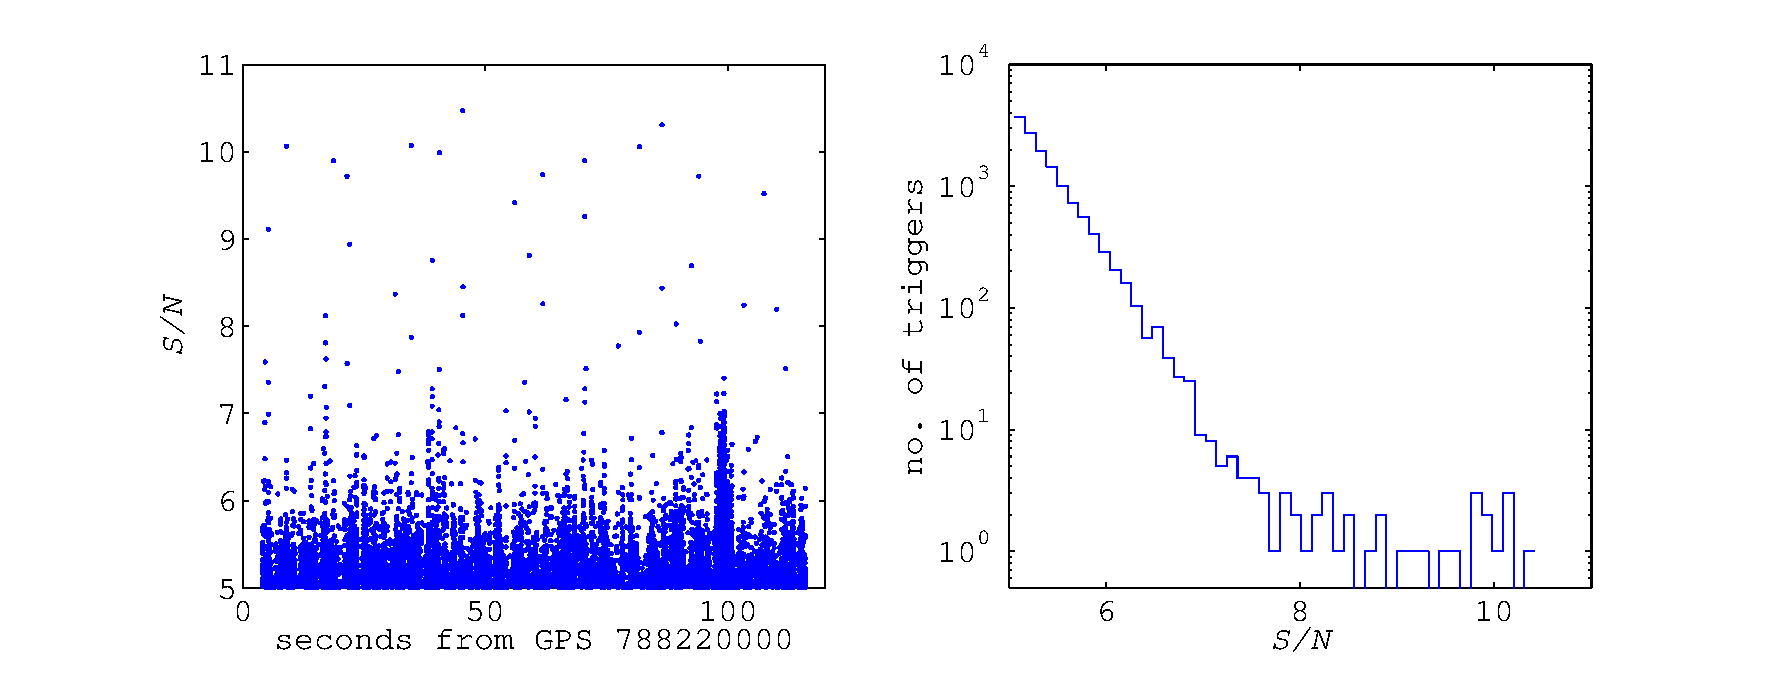
\includegraphics[width=0.8\textwidth]{figs/GEORingdownBgSNR}\caption{The distribution in $S/N$ of
events from the matched filtering algorithm for 120\,s of \geo data from GPS
788220000.}\label{GEORingdownBgSNR}
\end{center}
\end{figure}
Figure~\ref{GEORingdownBgSNR} also shows a large cluster of events around GPS 788220100 suggesting
some disturbance in the data. The tail in events extends further than that for H1 with a maximum
$S/N$ of 10.5. The large lines in the spectrum below 2000\,Hz are picked up strongly by the matched
filters (see figure~\ref{GEORingdownBgFreq}) with the disturbance at around GPS 788220100
contributing a significant amount of events in the upper half of the frequency range. The larger
number of lines in the spectrum makes it harder to veto out with confidence triggers that they were
caused by the lines, although it is obvious from figures~\ref{GEORingdownBgFreq} and
\ref{GEORingdownBgSNRVsFreq} that the largest $S/N$ triggers are caused  by a line at $\sim
1176$\,Hz.
\begin{figure}[!htbp]
\begin{center}
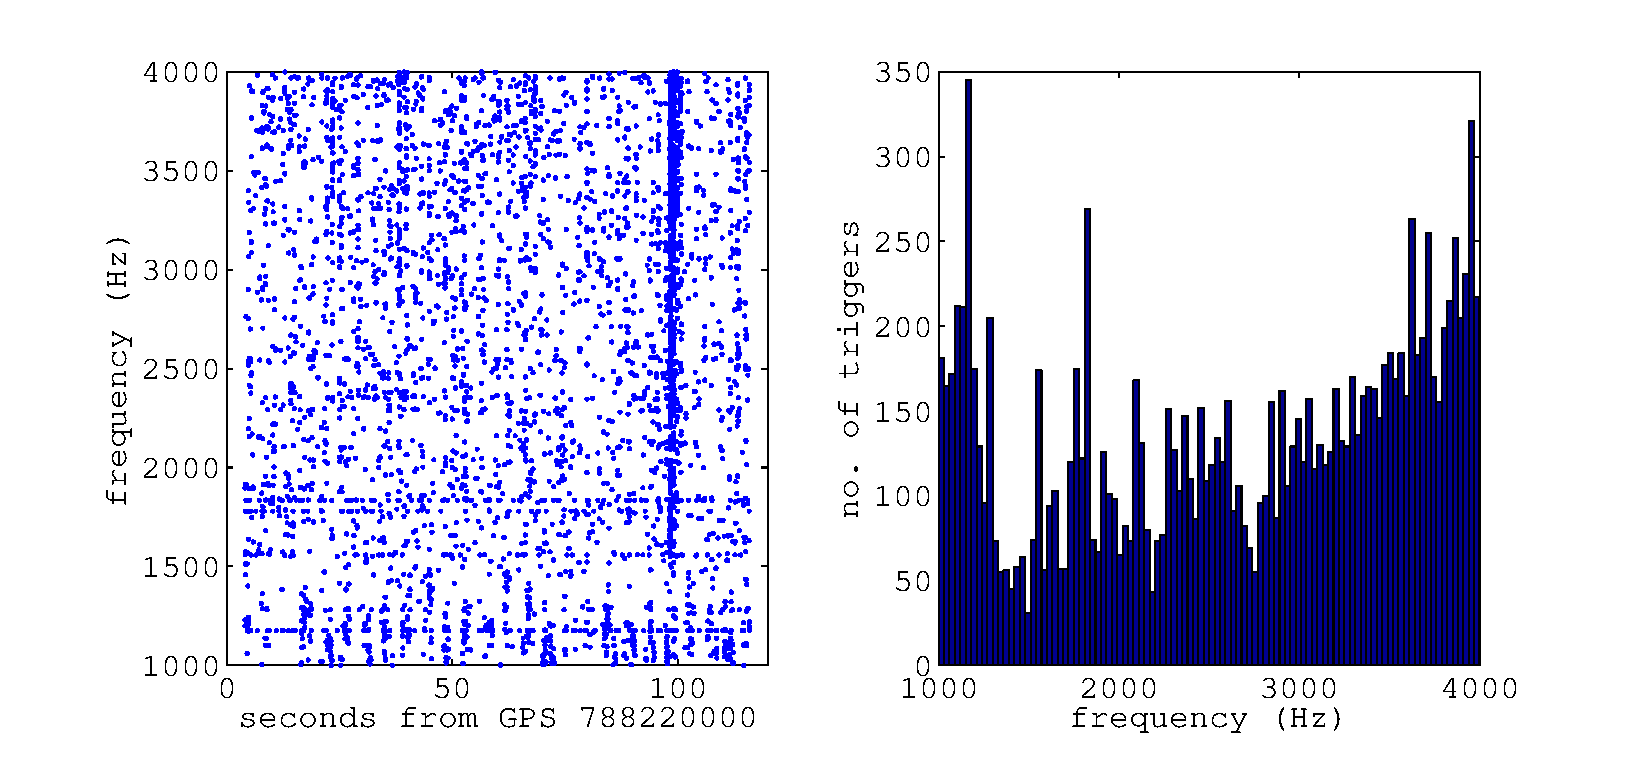
\includegraphics[width=0.8\textwidth]{figs/GEORingdownBgFreq}\caption{The distribution in frequency
of events from the matched filtering algorithm for 120\,s of \geo data from GPS
788220000.}\label{GEORingdownBgFreq}
\end{center}
\end{figure}
\begin{figure}[!htbp]
\begin{center}
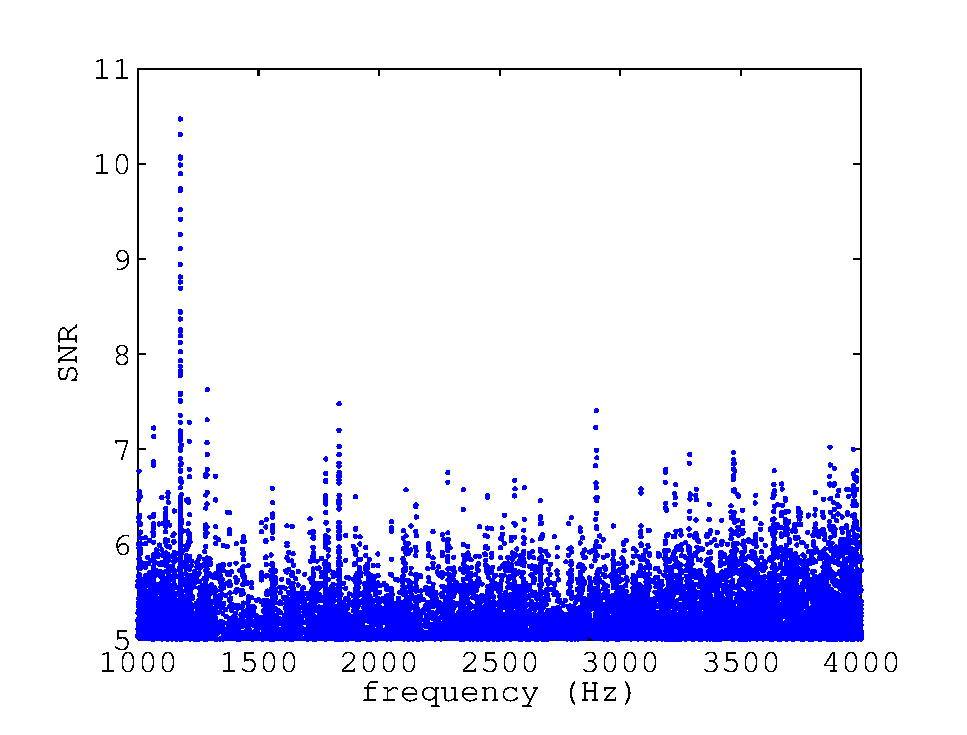
\includegraphics[width=0.6\textwidth]{figs/GEORingdownBgSNRVsFreq}\caption{The $S/N$ against
frequency for events from the matched filtering algorithm for 120\,s of \geo data from GPS
788220000.}\label{GEORingdownBgSNRVsFreq}
\end{center}
\end{figure}
From these background studies we can set thresholds on the $S/N$ at the time of the glitch, which we
will take as $> 8$ for H1 and $> 11$ for G\textsc{eo}\,600. 

After calculating a background threshold the matched filtering code was then run over the 120\,s
surrounding the time of the glitch, using the same parameters as for the background and simulated
noise studies. This provided 12\,537 events for \geo and 2126 events for H1 with $S/N > 5$. These
numbers are similar to those found on the background segments. No events rise above our thresholds
to give us any possible astrophysical triggers. In H1 the strongest events appear approximately 4.3
seconds before the time of the GRB, although these appears to be associated with the $\sim 1040$\,Hz
line feature becoming particularly strong around this time (see also the evidence analysis below). 

The most obvious veto for non-\gw signals is coincidence between detectors. Any \gw signal strong
enough should be visible in data from multiple detectors, with coincidence between arrival times
and amplitudes. This is most useful, and allows the the most stringent thresholds to be set, when
the detectors are of comparable sensitivity and are coaligned. For the detector pair we have, the
\geo data is approximately an order of magnitude less sensitive than H1, meaning that any signal
visible to both would be very strong in H1. The fact that the detectors are not coaligned also means
that they have different responses to the \gw polarisation, which additionally complicates things.
This factor will reduce the effective \gw amplitude for all except a source optimally positioned
directly above the plane of the detector. The polarisation of any signal is unknown, so any
coincidence threshold will have to be set with this reduction factor in mind for the less sensitive
detector. In our search for \gws from SGR\,1806-20 we know the source position and can therefore
calculate the detectors' responses to different source orientations. For \geo the factor
$\sqrt{F_+^2 + F_\times^2} = 0.84$ and for H1 it is 0.50. 

In our case where no triggers are seen above the set $S/N$ threshold no coincidence analysis is
possible. If we were to reduced our threshold too far however, say to the $S/N > 5$ used in the
background analyses, it would become difficult to use such a coincidence veto with the large number
of events seen leading to many accidental coincidences.

Many events will be produced by artifacts which do not in fact resemble our expected ring-down
waveform, as seen with the events from instrumental lines, so some method of vetoing these is
useful. In the matched filter search for inspiralling binaries a $\chi^2$ based discriminator is
used to veto such events \cite{Allen:2005}. The evidence based search below was originally conceived
as a possible waveform consistency veto, with the hope of combining the matched filter results and
evidence searches.

\subsubsection{Evidence search}
This method is most efficient if the ring-down signal begins at the start of the data section being
studied. It would take too long computationally, and be unnecessary, to implement such a search from
the start of each consecutive sample at 16\,384\,Hz. A time step of $\frac{1}{8}$\,s and a data
length of 1\,s was chosen as a reasonable duration to catch the shortest events and span the longest
events. The overlap between consecutive data segments (0.875\,s) means that the evidence for each is
not truly independent and could be correlated. 

As with the matched filtering search we want to gauge some background level for this method. It was
seen in figure~\ref{evidenceNoise} that Gaussian noise will give a certain background level, but
again real data needs studying. For this purpose the same section of off-source data as used in the
matched filter search was studied. The data for both H1 and \geo was high-pass filtered to remove
low frequency noise before applying the evidence finding algorithm. The first evidence value from
each data segment analysed was ignored due to contamination from the filter response, although
overlapping of data in the analysis meant that all the time was covered. The evidence for 4776
overlapping segments from H1 (covering 597\,s) from GPS 788220000 can be seen in
figure~\ref{H1EvidenceOffsource}.
\begin{figure}[!htbp]
\begin{center}
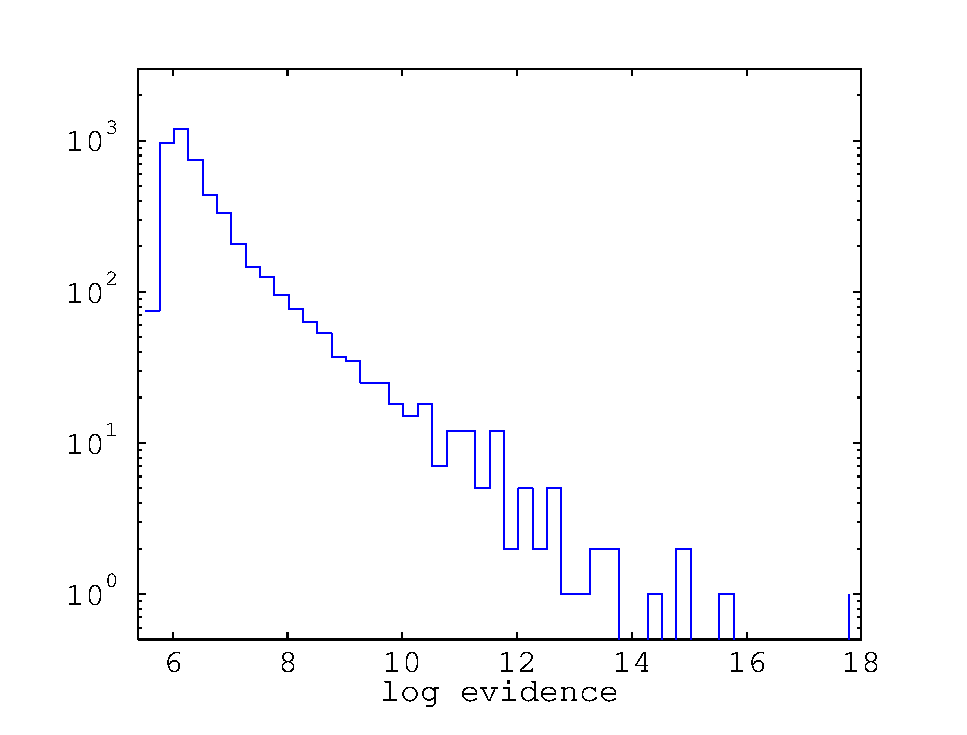
\includegraphics[width=0.6\textwidth]{figs/H1EvidenceOffsource}\caption{The evidence
of a ring-down signal in H1 data from GPS 788220000 for 597\,s.}\label{H1EvidenceOffsource}
\end{center}
\end{figure}
The H1 data was uncalibrated and whitened so certain spectral features were suppressed. As with
the test on Gaussian noise figure~\ref{H1EvidenceOffsource} shows the value of $\log{\rm evidence}$
clustering around 6, with a mean of 6.55. For real data a larger tail to the evidence is present
suggesting more spectral contamination within the frequency band. This can be seen when looking at
the posterior pdf of frequency at times when the evidence is highest, for example at the time of the
maximum value of $\log{\rm evidence} = 17.9$. From the studies on Gaussian noise such high evidence
values would suggest the presence of a signal, but figure~\ref{H1OffsourcePosterior} shows that this
value is almost entirely due to the spectral line at $f \sim 1045$\,Hz, as seen in the matched
filter studies above. This was confirmed as a spectral line feature, and not an actual signal, by
studying spectra from periods long before the GRB occurred. This means that without removing this
spectral feature a far higher threshold on the evidence than is suggested by Gaussian noise studies
is needed. We will set a threshold of $\log{\rm evidence} > 20$ for the data around the GRB.
\begin{figure}[!htbp]
\begin{center}
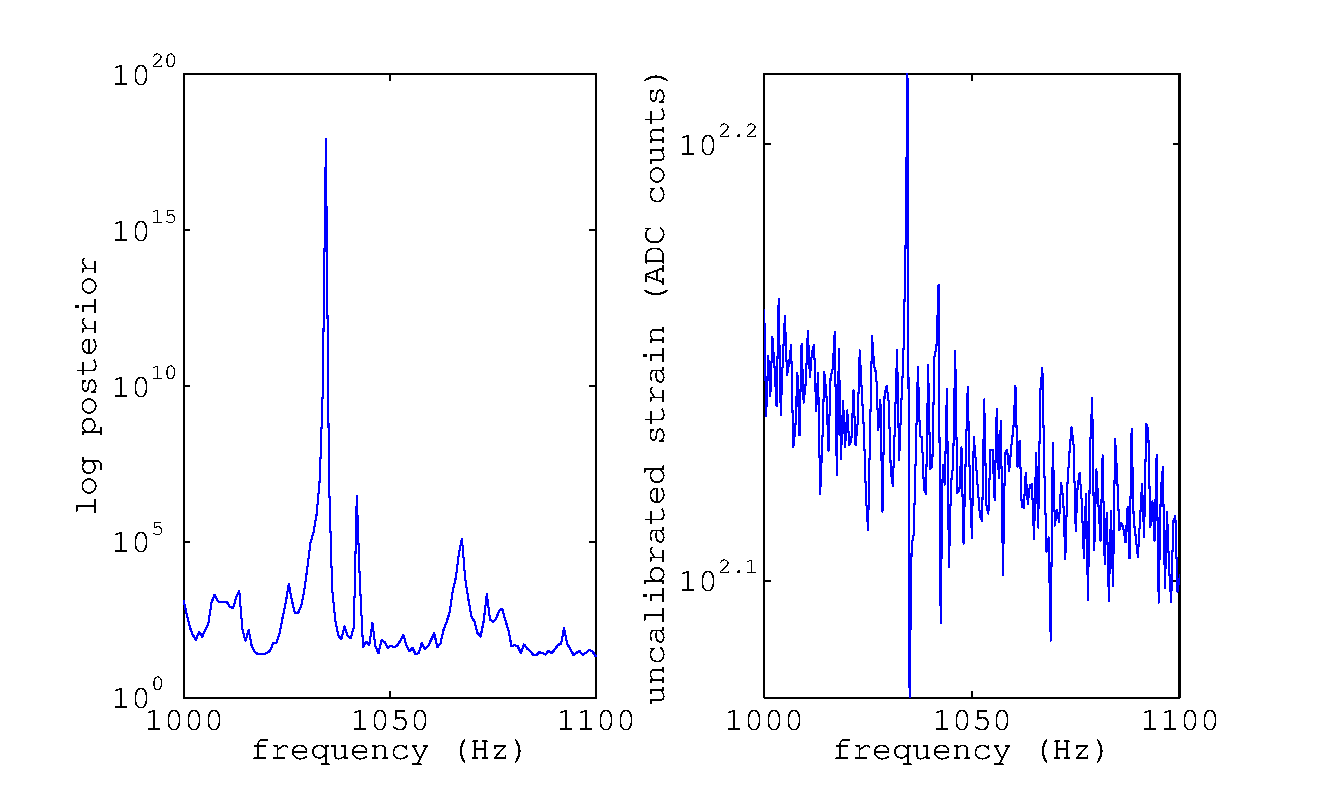
\includegraphics[width=0.8\textwidth]{figs/H1OffsourcePosterior}\caption[Comparision of
posterior pdf with an FFT at the time of highest evidence.]{Comparison of the posterior pdf of
frequency from the Bayesian method for the data giving the highest background evidence value and an
FFT of the same data.}\label{H1OffsourcePosterior}
\end{center}
\end{figure}

The search performed on the 120\,s of data around the time of the GRB produces evidence values
similar to those in the background (see figure~\ref{H1EvidenceOnsource}). There are spikes in the
evidence which, as with the background data, are caused by the spectral lines, like the matched
filter events. The highest value of $\log{\rm evidence} = 18.3$ occurs $\sim 4.3$\,s before the
GRB, at the same time as the highest $S/N$ matched filter event, suggesting the same source. The
frequency posterior and spectrum have been examined showing the $f \sim 1045$\,Hz spectral line to
be particularly strong at this time. None of these spikes crosses our $\log{\rm evidence} > 20$
threshold.
\begin{figure}[!htbp]
\begin{center}
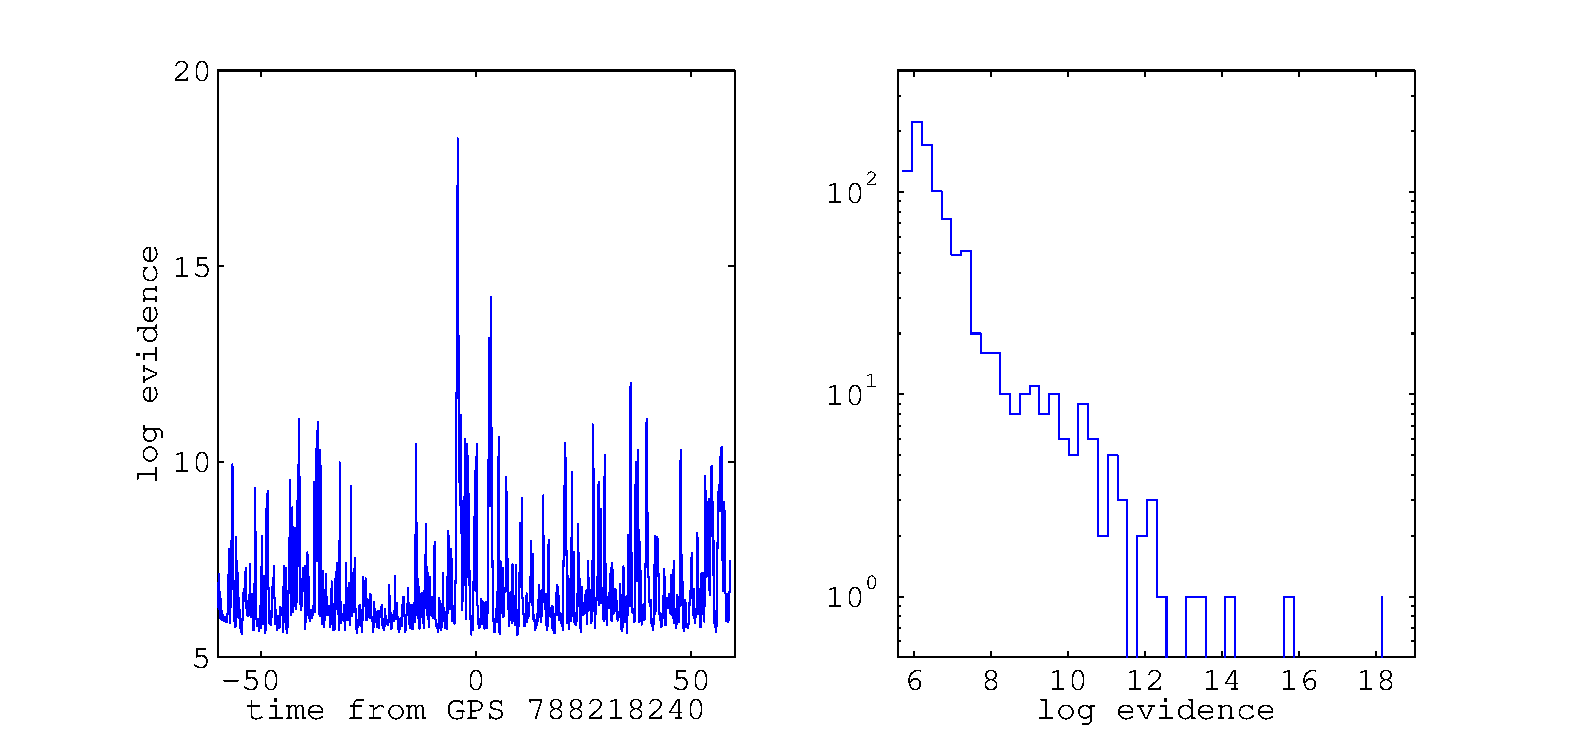
\includegraphics[width=0.8\textwidth]{figs/H1EvidenceOnsource}\caption{The evidence
of a ring-down signal in H1 data from for 120 seconds around the GRB time of GPS
788218240\,s.}\label{H1EvidenceOnsource}
\end{center}
\end{figure}

Using studies of the efficiency of this algorithm it still might prove useful in vetoing H1
triggers above the original matched filter $S/N$ threshold of 5. To do this a simulation has been
performed in which 4000 ring-down signals of varying amplitude, frequency and decay time have been
injected into Gaussian noise and the $S/N$ and evidence calculated. These signals have a start time
that varies randomly between $0-\frac{1}{8}$\,s to reproduce the time step between consecutive
segments used in the actual analysis. The evidence as a function of $S/N$ is plotted in
figure~\ref{evidenceVsSNR}. The flat roof on the evidence is an artifact of the evidence code, which
sets the posterior value equal to $e^{230}$ ($\approx 10^{100}$) if it is greater than this, due to
it otherwise getting outside the dynamic range allowed by double precision.
\begin{figure}[!htbp]
\begin{center}
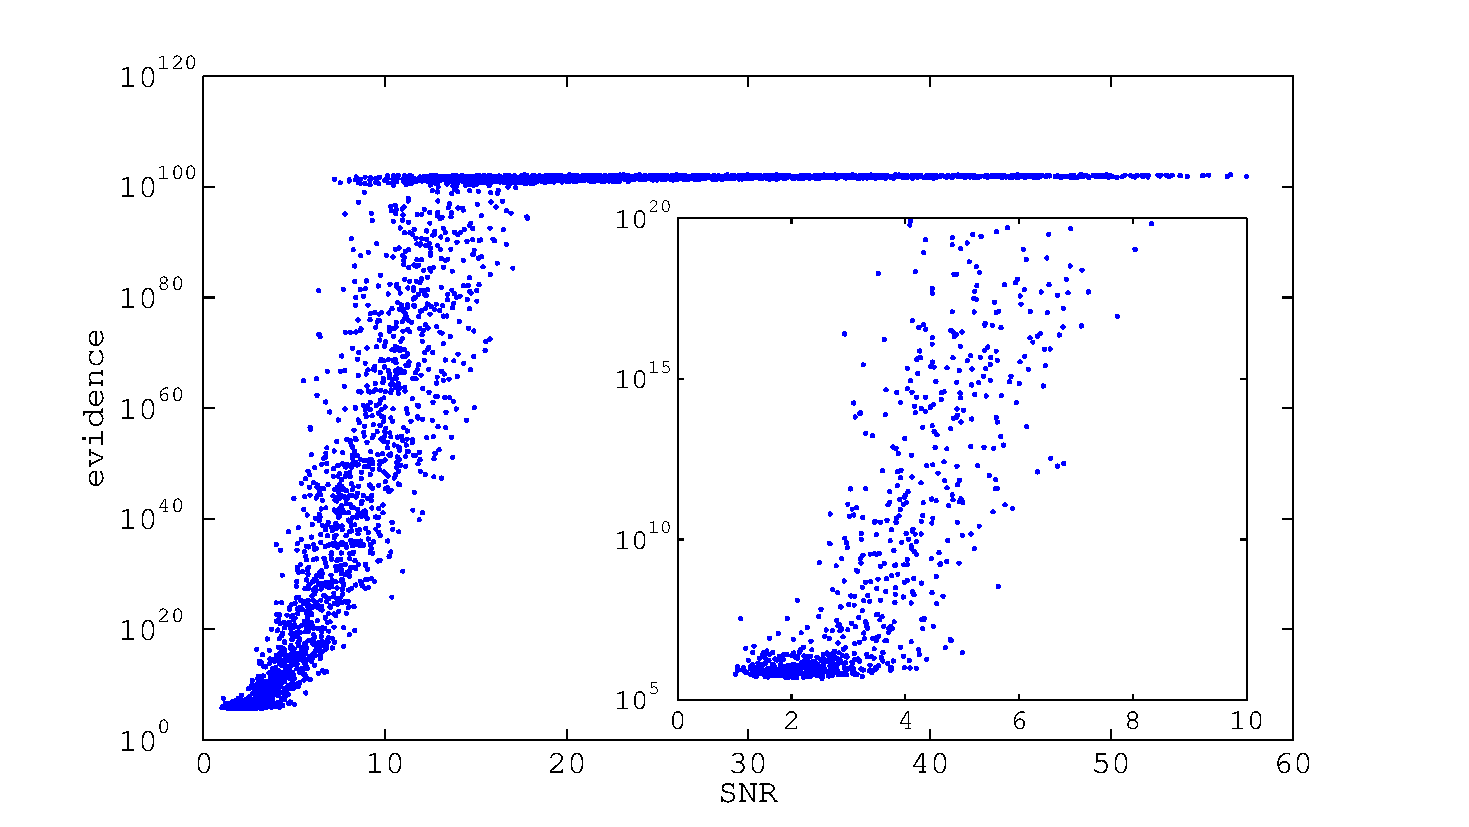
\includegraphics[width=0.6\textwidth]{figs/evidenceVsSNR}\caption{The evidence for ring-down
signals against the signal $S/N$ for 4000 simulated ring-down signals injected into Gaussian
noise.}\label{evidenceVsSNR}
\end{center}
\end{figure}
We need to set some evidence limit for which we believe the code has truly seen the signal. From our
studies on Gaussian noise with no signal injected (see figure~\ref{evidenceNoise}) we can see that
evidence values can reach out to nearly $10^{8.5}$ with a mean of $\sim 10^{6}$, so conservatively
we can say that we see a signal if the evidence is $> 10^{10}$. From figure~\ref{evidenceVsSNR} this
means that we see all the events with $S/N$ $> 5.63$. Using this evidence threshold we can plot the
efficiency of the search (see figure~\ref{evidenceEfficiency}) and see that above an $S/N$ of 6 we
see all triggers and below an $S/N$ of 2.5 we see no triggers.
\begin{figure}[!htbp]
\begin{center}
\includegraphics[width=0.6\textwidth]{figs/evidenceEfficiency}\caption{The efficiency of the
evidence search for different signal $S/N$s.}\label{evidenceEfficiency}
\end{center}
\end{figure}

It has been seen that lines in the spectra can produce a large evidence value even though they are
not ring-downs. To estimate how this could effect the analysis we have done a simulation by
injecting 2000 sinusoids with random frequency and amplitude parameters into Gaussian noise. The
evidence against $S/N$ is plotted in figure~\ref{evidenceVsSNRForSins} and shows that, using our
evidence threshold of above $10^{10}$ being a signal detection, all sinusoids with $S/N$ $\gtrsim
6.7$ will be picked up. This shows that the evidence as it is currently implemented, using short
1\,second stretches of data, is not promising as a method of distinguishing ring-downs from lines,
and possible extensions to this end are discussed below.
\begin{figure}[!htbp]
\begin{center}
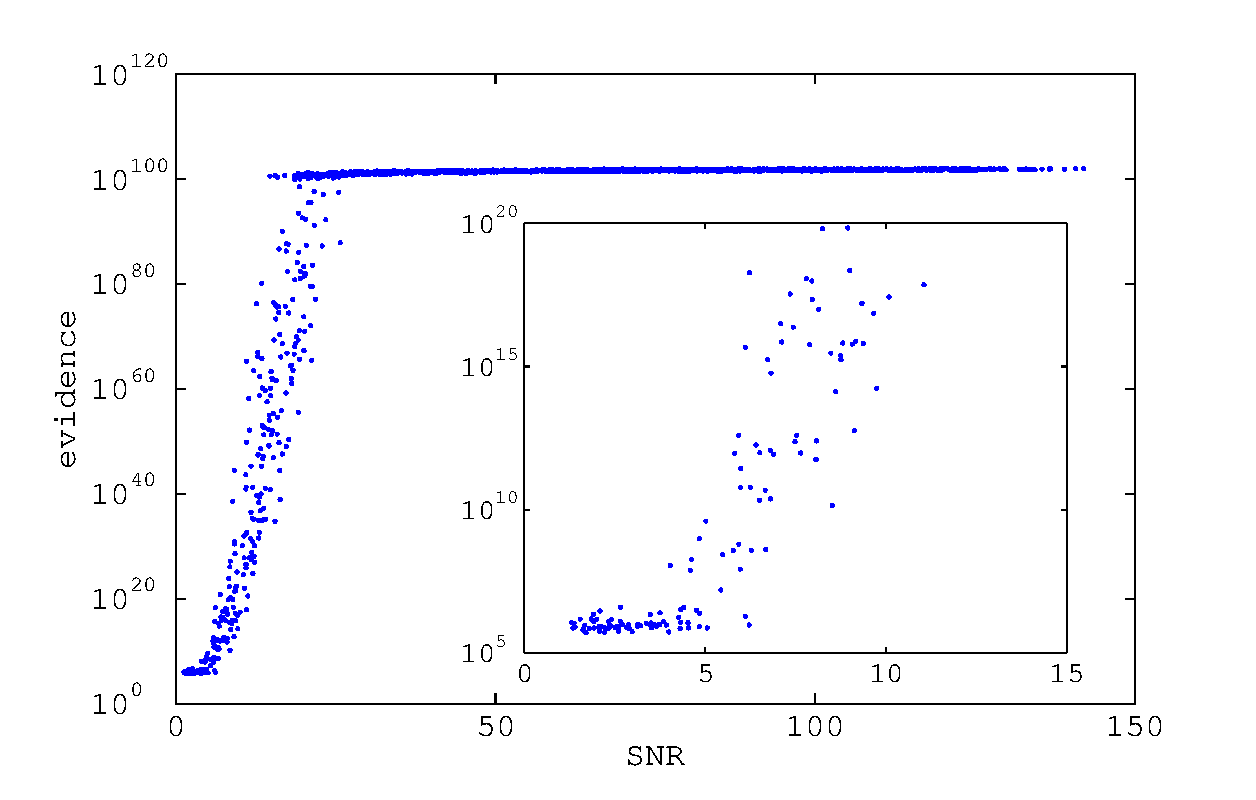
\includegraphics[width=0.6\textwidth]{figs/evidenceVsSNRForSins}\caption{The evidence for ring-down
signals against $S/N$ for 2000 simulated sinusoids injected into Gaussian
noise.}\label{evidenceVsSNRForSins}
\end{center}
\end{figure}

Detector data can also contain many transient $\delta$-function like events, so a simulation has
been performed to see whether these trigger our evidence algorithm above the level of Gaussian
noise. 2000 $\delta$-functions have been in injected into Gaussian noise with a range of amplitudes
(see figure~\ref{evidenceVsSNRForDelta}) and it can be seen that all evidence values are well
below our evidence threshold of $10^{10}$ and cover a very similar range to those from pure noise
(see figure~\ref{evidenceNoise}). Such signals do not seem to affect our algorithm in any way. In
the future other types of signal such as ring-ups or chirps will be tested.
\begin{figure}[!htbp]
\begin{center}
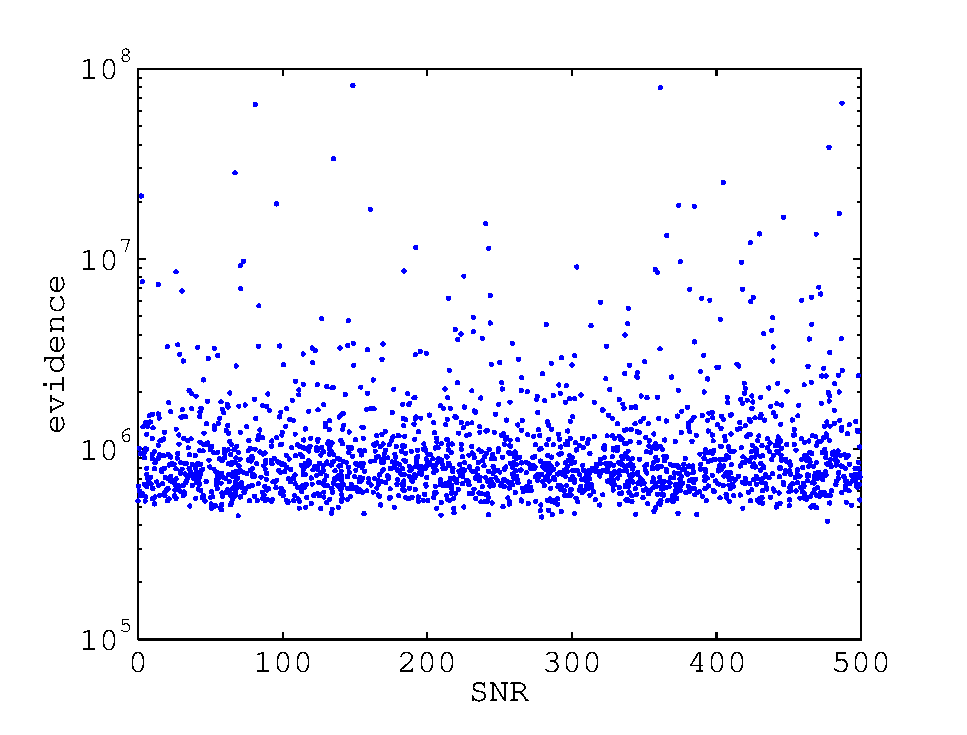
\includegraphics[width=0.6\textwidth]{figs/evidenceVsSNRForDelta}\caption{The evidence for ring-down
signals against $S/N$ for 2000 simulated $\delta$-functions injected into Gaussian
noise.}\label{evidenceVsSNRForDelta}
\end{center}
\end{figure}

For \geo the data is calibrated and contains very strong calibration lines within our band of
study. Without the removal of these lines it makes our evidence studies almost useless as they
completely swamp the evidence. This can be seen in the frequency posterior pdf for a section of
\geo data (see figure~\ref{GEORingdownPosterior}) in which almost all the probability is at the
frequencies of the spectral lines shown in figure~\ref{GEOSpectrumRingdownSearch}.
\begin{figure}[!htbp]
\begin{center}
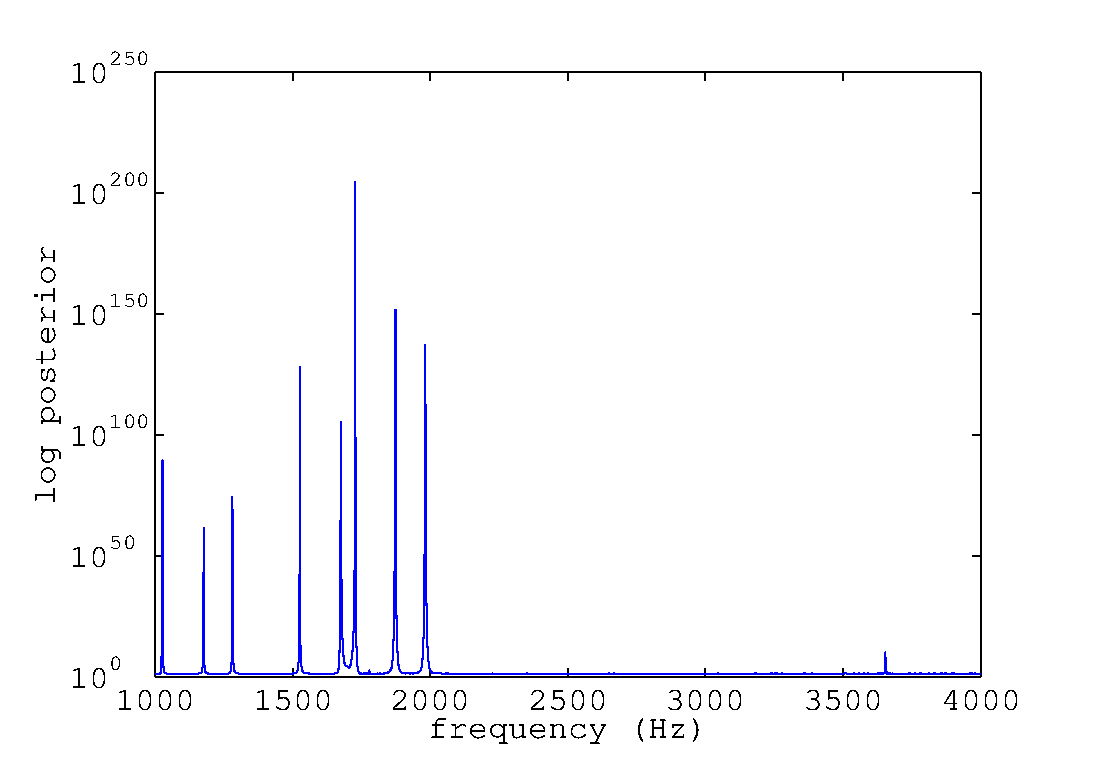
\includegraphics[width=0.6\textwidth]{figs/GEORingdownPosterior}\caption{ The frequency posterior
for ring-down signals in a section of \geo data.}\label{GEORingdownPosterior}
\end{center}
\end{figure}
These excessively large probability values also make it hard to calculate a true value of the
evidence as they will be out of the range of the double precision variable in the code. For all the
\geo data analysed this limit on the evidence is reached just from the spectral lines and can
therefore tell us nothing about the presence of ring-down signals.

These studies show that the Bayesian evidence method, as currently implemented, does not
sufficiently discriminate against non-decaying sinusoids. In the absence of there being any
better alternative hypothesis the code will take sinusoids as the nearest thing to a ring-down
signal. In our implementation this happens because of the short 1\,s time of the data segments
being used. It was shown that for $\delta$-functions, which are essentially very short ring-downs,
the 1\,s time stretch is long enough by far that the probability that they are within our range of
$\tau$ becomes very small. If the segment times were increased then the probability of long duration
sinusoids being within our $\tau$ range should also be small, although a very preliminary test shows
that this timescale needs to be $\gg 100$\,s.

There are several possible options which could be implemented in the future to help make the
algorithm more robust against non-ring-down signals. One way, as just stated, would be to increase
the length of data segments. This could become computationally expensive, although if the
marginalisation can be performed analytically, or at least approximated analytically, then this
would become far more practical. Another obvious method is to use notch filters to remove known
instrumental lines e.g. calibration lines, suspension violin modes. A more complex method would be
to extend the Bayesian analysis to include non-decaying sinusoids in some way that they can be
excluded. This would mean that a number of sinusoidal models, $N$, could be included
\begin{equation}
y(t) = A\sin{(2\pi{}ft+\phi_0)}e^{-(t-T_0)/\tau} + \sum_{i=1}^N B_i\sin{(2\pi{}f_it+\phi_i)}, 
\end{equation}
which would provide a better model for any line features to assume, leaving the ring-down model free
to estimate the presence of ring-down signals alone. Along similar lines you could instead have $N$
ring-down models and veto any with values of $\tau$ outside our range, which would include
non-decaying sinusoids with $\tau = \infty$, or transient delta functions with $\tau \to 0$. Or a
model with $N_1$ ring-downs and $N_2$ sinusoids. The parameter $T_0$ could also be searched
over, eliminating the need for large numbers of overlaps between successive data segments. This
could become computationally expensive for data with many lines and might need to be implemented
using an MCMC approach. This would be similar to a method being developed to estimate the large
number white dwarf binary system in LISA data \cite{Umstatter:2005}.

\subsection{Results}
The aim of this search was to find out whether or not any ring-down \gw burst was seen associated
with the $27^{\rm th}$ December 2004 GRB and in that the result is negative. We are however, able to
set an upper limit on \gw emission by making use of our $S/N$ thresholds. These results only make
use of the matched filter search.

For \geo data no triggers were seen above our $S/N$ threshold of 11 across our entire frequency
range, so using the antenna response of 0.84 we can produce an upper limit on the effective strain
from our source as given by figure~\ref{GEORingdownUL}.
\begin{figure}[!htbp]
\begin{center}
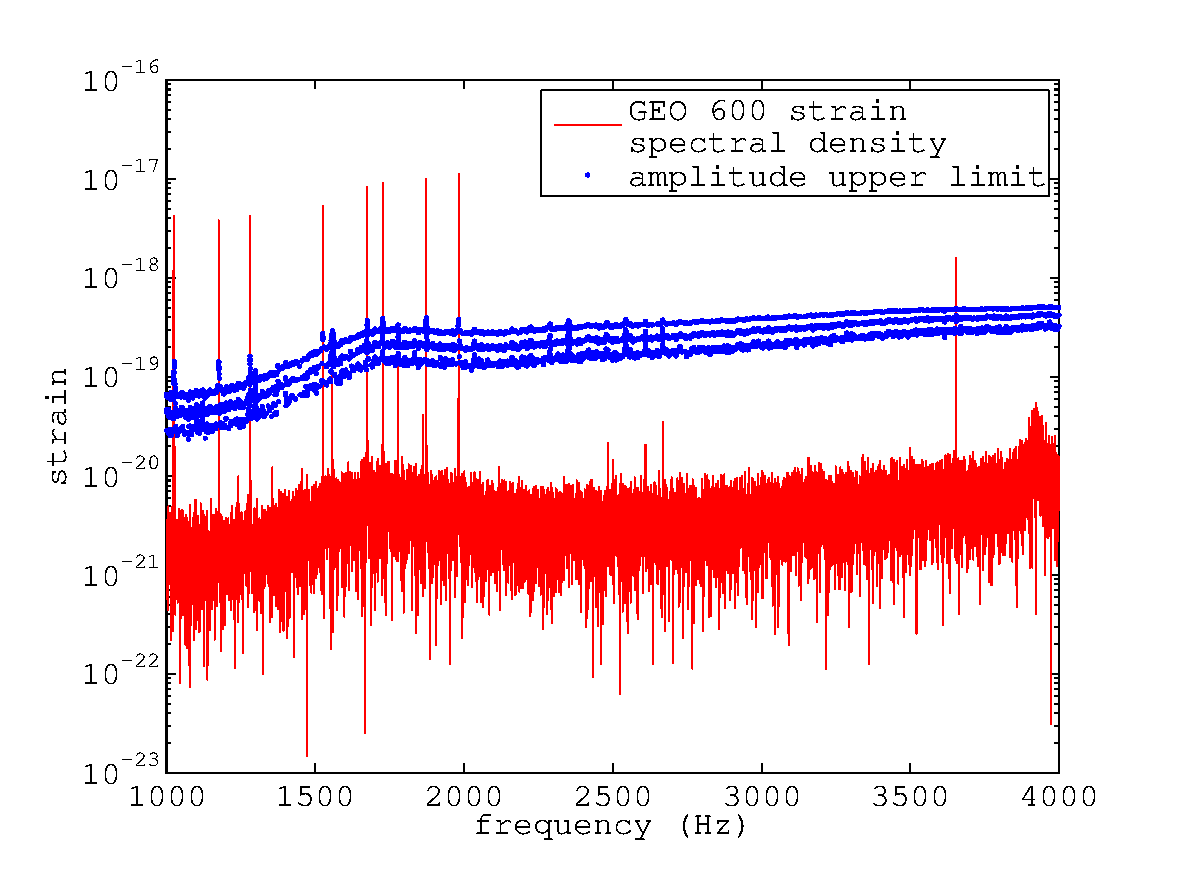
\includegraphics[width=0.6\textwidth]{figs/GEORingdownUL}\caption[The upper limit on
effective amplitude of ring-down signals from SGR\,1806-20 using \geo data.]{The upper limit on
effective amplitude of ring-down signals from SGR\,1806-20 using \geo data shown along with an
estimate of the noise spectral density.}\label{GEORingdownUL}
\end{center}
\end{figure}
For the H1 data no triggers were seen above our $S/N$ threshold of 8 across the entire frequency
range, so using the antenna response of 0.50 we can produce an upper limit on the effective strain
as given in figure~\ref{H1RingdownUL}. The H1 data gives the most stringent upper limits with them
ranging from $h_0 \sim 10^{-20}$ at the low frequency end to $h_0 \sim 10^{-19}$ at the high
frequency end. The $S/N$, and therefore amplitudes, will have an error of about 5\% from the 10\%
filter mis-match used in the matched filtering. These results are plotted in terms of an upper
limit on the energy emitted (via equation~\ref{RingAmplitude} using $r = 15$\,kpc) in
figure~\ref{H1RingdownEnergyUL}.
\begin{figure}[!htbp]
\begin{center}
\includegraphics[width=0.6\textwidth]{figs/H1RingdownUL}\caption[The upper limit on the effective
amplitude of ring-down signals from SGR\,1806-20 using H1 data.]{The upper limit on the effective
amplitude of ring-down signals from SGR\,1806-20 using H1 data shown along with an estimate of the
noise spectral density.}\label{H1RingdownUL}
\end{center}
\end{figure}
This gives an upper limit on the energy emitted ranging from $E \sim 2\ee{-6}\,{\rm M}_{\odot}c^2$
at the low frequency end to $E \sim 5\ee{-4}\,{\rm M}_{\odot}c^2$ at the high frequency end (see
figure ~\ref{H1RingdownEnergyUL}). The results at low frequency beat those given in Baggio {\it et
al.} (2005) \cite{Baggio:2005} although do not quite extend into their frequency range. The results
are still about 3 orders of magnitude greater than the upper limit from spin-down argument set above
with $h_{\rm eff} < 10^{-23}$, but are into the range of amplitudes expected from new born neutron
stars. Thus we are starting to get into the range of some interesting astrophysics.
\begin{figure}[!htbp]
\begin{center}
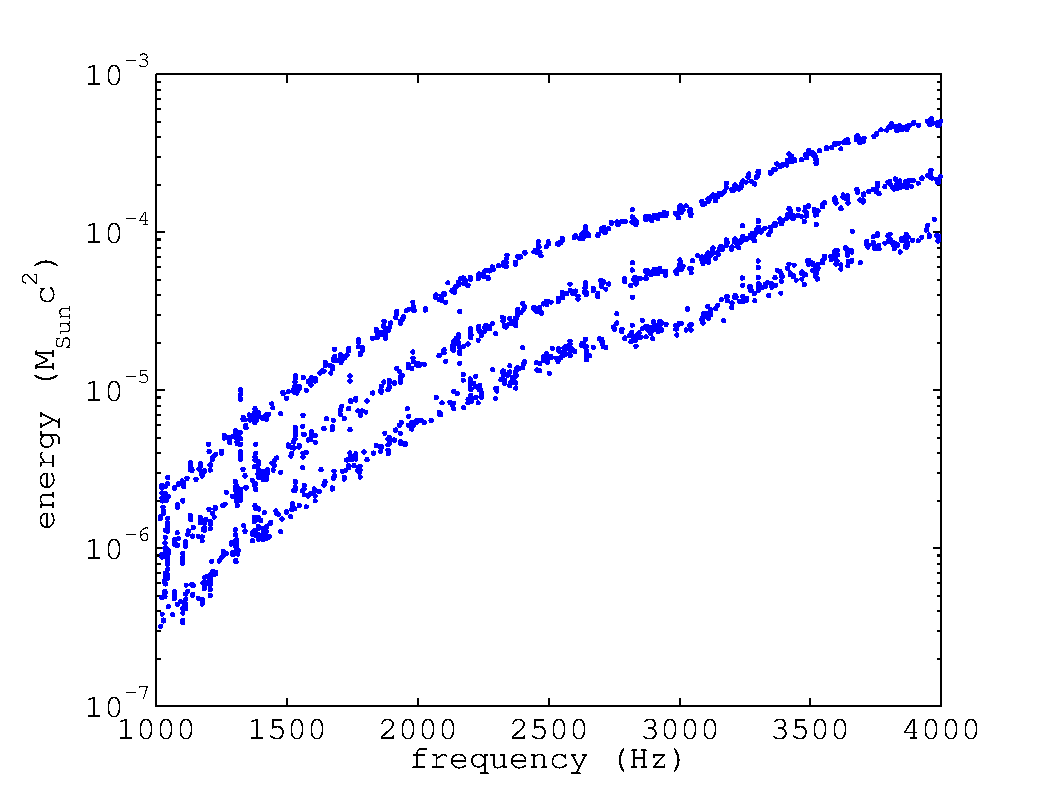
\includegraphics[width=0.6\textwidth]{figs/H1RingdownEnergyUL}\caption{The upper limit
on energy of ring-down signals from SGR\,1806-20 using H1 data.}\label{H1RingdownEnergyUL}
\end{center}
\end{figure}

Here we have performed and described only a preliminary analysis of this data, with much work still
needed. The data can be made more effective for this study with some line removal strategy. A
background coincidence analysis can be performed to attempt to reduce the $S/N$ threshold. The
matched filter search and evidence search will also be combined to provide increased confidence in
the result. Therefore a more detailed analysis of the data could potentially push down the upper
limits stated above. 

\section{Other pulsar ring-down studies}
\subsection{Crab and Vela pulsar glitches}
The Crab and Vela pulsars have both glitched during periods when at least one interferometer has
been taking data. For the Crab pulsar these glitches have been on $3^{\rm rd}$ March, $6^{\rm th}$
September and $12^{\rm th}$ November 2004 \cite{CrabEphemeris}. For the Vela pulsar a glitch with a
fractional change in period of $2.1\ee{-6}$ was observed on $7^{\rm th}$ July 2004
\cite{Dodson:2004}. At present this data has yet to be dug out and analysed and although a
detection is very unlikely these could provide some interesting upper limits.
